\documentclass[
    a4paper, % Stock and paper size.
    10pt, % Type size.
    %article,
    oneside, 
    onecolumn, % Only one column of text on a page.
    openright, % Each chapter will start on a recto page.
    % openleft, % Each chapter will start on a verso page.
    % openany, % A chapter may start on either a recto or verso page.
    ]{memoir}
\usepackage[utf8]{inputenc}
\usepackage[T1]{fontenc}
\usepackage{lmodern}
\usepackage[final]{microtype}
\usepackage[dvips]{graphicx}
\usepackage{xcolor}
\usepackage{pgfplots}
\usepackage{tikz}
\usepgfplotslibrary{groupplots}
\usepackage{epstopdf}
\usepackage{multirow}
\usepackage{multicol}
\usepackage[ruled,vlined]{algorithm2e}
\usepackage{placeins}
\usepackage{amsfonts} 

\usetikzlibrary{patterns}
\usetikzlibrary{positioning}
\usepackage[mode=buildnew]{standalone}

\graphicspath{{automated_graphs/}{.}{images/}{images/morphmask_denoise2_erode2_MyoSegmenTUM_043}}


\usetikzlibrary{calc}
\usepackage[font=small]{caption}
%\usepackage{times}

% Comment in final version
\usepackage{todonotes}
\usepackage{soul}
\usepackage{pdfpages}

%\usepackage[margincaption,outercaption,ragged,wide]{sidecap}
\usepackage[margincaption,ragged]{sidecap}
\sidecaptionvpos{figure}{t} 
\sidecaptionvpos{table}{t}

\usepackage[
breaklinks=true,colorlinks=true,
%linkcolor=blue,urlcolor=blue,citecolor=blue,% PDF VIEW
linkcolor=black,urlcolor=black,citecolor=black,% PRINT
bookmarks=true,bookmarksopenlevel=2]{hyperref}

\usepackage{geometry}
% PDF VIEW
% \geometry{total={210mm,297mm},
% left=25mm,right=25mm,%
% bindingoffset=0mm, top=25mm,bottom=25mm}
% PRINT
% \geometry{total={210mm,297mm},left=20mm,right=50mm,bindingoffset=10mm, top=25mm,bottom=25mm}

% Code from https://tex.stackexchange.com/questions/275565/tufte-layout-in-painless-memoir

% Start code

% MEMOIR LAYOUT
\setlength{\baselineskip}{14pt}
\setlength{\normalbaselineskip}{14pt}

% GEOMETRY
\settrims{0pt}{0pt}
\settypeblocksize{50\baselineskip}{120mm}{*}
\setlrmargins{16.0mm}{*}{*} % 24.8 mm
\setulmargins{25.0mm}{*}{*} % 27.4 mm
\setheadfoot{\baselineskip}{\baselineskip}
\setheaderspaces{*}{2\baselineskip}{*}
\setmarginnotes{11.3mm}{49mm}{\onelineskip} % was 8.2 and 49.4
\checkandfixthelayout


% TEXT
% ragged2e provides ragged justification with hyphenation
\RequirePackage{ragged2e}
\AtBeginDocument{\RaggedRight}
\setmpjustification{\RaggedLeft}{\RaggedRight}
\setlength{\RaggedRightParindent}{1.0pc}
\setlength{\parindent}{1pc}
\setlength{\parskip}{0pt}
% linespacing ~ 14pt
\linespread{1.17}

% text styling of all side footnotes
\renewcommand{\footnotesize}{\fontsize{8pt}{8pt}\selectfont}
\renewcommand{\foottextfont}{\footnotesize}
% styling and placement of mark
\footmarkstyle{{#1. }}
\setlength{\footmarkwidth}{0em}
\setlength{\footmarksep}{-\footmarkwidth}
% memoir command - do all footnotes in margin
\footnotesinmargin


% SIDECAPTIONS
\setsidecaps{\marginparsep}{\marginparwidth}
\sidecapmargin{outer}
\setsidecappos{t}
\renewcommand*{\sidecapstyle}{%
\captionnamefont{\foottextfont\scshape\footnotesize}
\ifscapmargleft
\captionstyle{\RaggedLeft\footnotesize\foottextfont}%
\else
\captionstyle{\RaggedRight\footnotesize\foottextfont}%
\fi}

% FULLWIDTH environment
% The following code should be used *after* any changes to the margins and
% page layout are made (e.g., after the geometry package has been loaded).
\newlength{\fullwidthlen}
\setlength{\fullwidthlen}{\marginparwidth}
\addtolength{\fullwidthlen}{\marginparsep}

% \newlength{\fullwidthlen}
% \setlength{\fullwidthlen}{\marginparwidth}
% \addtolength{\fullwidthlen}{\marginparsep}

\newenvironment{fullwidth}{%
  \begin{adjustwidth*}{}{-\fullwidthlen}%
}{%
  \end{adjustwidth*}%
}


% End code

%

%\OnehalfSpacing
%\linespread{1.3}

% disable by disabling the todo notes
\makeatletter
 \if@todonotes@disabled
 \newcommand{\hlnote}[2]{#1}
 \else
 \newcommand{\hlnote}[2]{\todo{#2}\texthl{#1}}
 \fi
 \makeatother

%%% CHAPTER'S STYLE
%\chapterstyle{bianchi}
%\chapterstyle{ger}
\chapterstyle{dash}

%\chapterstyle{madsen}
%\chapterstyle{ell}
%%% STYLE OF SECTIONS, SUBSECTIONS, AND SUBSUBSECTIONS
\setsecheadstyle{\Large\bfseries\sffamily\raggedright}
\setsubsecheadstyle{\large\bfseries\sffamily\raggedright}
\setsubsubsecheadstyle{\bfseries\sffamily\raggedright}


%%% STYLE OF PAGES NUMBERING
\pagestyle{companion}\nouppercaseheads 
%\pagestyle{headings}
%\pagestyle{Ruled}
%\pagestyle{plain}
\makepagestyle{plain}
\makeevenfoot{plain}{\thepage}{}{}
\makeoddfoot{plain}{}{}{\thepage}
\makeevenhead{plain}{}{}{}
\makeoddhead{plain}{}{}{}

%%% For parts with abstracts on the page

\usepackage{xpatch}

\makeatletter
\xpatchcmd{\part}{\null\vfil}{\vspace*{.1\textheight}}{}{}

\providecommand{\abstractname}{Content of this part}
\newenvironment{partwithabstract}
  {\begingroup\let\@endpart\relax\part@withabstract}
  {\endquotation\endgroup\@endpart}
\newcommand{\part@withabstract}{\@dblarg\part@@withabstract}
\def\part@@withabstract[#1]#2{%
  \part[#1]{#2}%
  \vfil
  \begin{center}\bfseries\abstractname\vspace{-.5em}\vspace{\z@}\end{center}
  \quotation
}
\makeatother

% squares for color indication

\newrobustcmd*{\mycircle}[1]{\tikz{\filldraw[draw=#1,fill=#1] (0,0) circle [radius=0.1cm];}}
\definecolor{colL1}{rgb}{0.8, 0.8, 0.24528301886792458}
\definecolor{colL2}{rgb}{0.6, 0.6, 0.5744680851063829}
\definecolor{colL3}{rgb}{0.3999999999999999, 0.4, 0.8}
\definecolor{colL4}{rgb}{0.27610394265232974, 0.19999999999999996, 0.4}
\definecolor{colL5}{rgb}{0.0, 0.0, 0.0}

\maxsecnumdepth{subsection} % chapters, sections, and subsections are numbered
\maxtocdepth{subsection} % chapters, sections, and subsections are in the Table of Contents

\usepackage[backend=biber]{biblatex}
\addbibresource{bibreferences.bib}

%% make a glossary
\usepackage[acronym, xindy]{glossaries}
\makeglossaries


\newglossaryentry{weaklysupervisedl}
{
        name={Weakly Supervised},
        description={Weakly supervised machine learning where the ground truth labels are only partially available. 
        In the context of image segmentation, this can mean that the labels are only provided at image level or that point level annotation in the image is provided.
        The model is trained on incomplete labels, the desired result remains the complete segmentation of the image.
        Just like in the case of \textit{Fully Supervised Learning} the objective is to model the relationship between an \textit{input} and an \textit{output}. 
        Due to the labels being incomplete, there is a stronger need to identify the internal structure of the data, as is the case for \textit{Unsupervised learning}.
        }
}

\newglossaryentry{segmentation}{
        name={Segmentation},
        description={
                The \textit{segmentation} problem in machine vision consists of the classification of each individual pixel or voxel. 
                The problem of \textit{semantic} segmentation is to detect, for each pixel, the object category it belongs to. 
                \textit{Instance} segmentation digs deeper. It identifies for each pixel the object instance it belongs to.
                The difference is that it differentiates between two objects of the same object category in the picture. 
                }
        }

\newglossaryentry{groundtruth}{
        name={Ground Truth},
        description={
                The \textit{Ground Truth} is a term used in machine learning to indicate the ideal expected result. 
                In the context of Instance Segmentation, the ground truth is the true class of every pixel or voxel. 
        }
        }

\newglossaryentry{unsupervisedl}
{
        name={Unsupervised},
        description={
                In an \textit{Unsupervised} machine learning problem, no labels are present. 
                The aim is not to model the relationship between an \textit{input} and an \textit{output}, the aim is to model the structure of the data.
                Frequent applications of these techniques are clustering and dimensionality reduction of data. 
                }
}

\newglossaryentry{supervisedl}
{
        name={Supervised},
        description={
                (Fully) Supervised Machine Learning task where target labels are present. 
                The objective of these problems is to model the relationship between an \textit{input} and an \textit{output}.
                }
}

\newglossaryentry{tomography}
{
        name={Tomography},
        description={
                Imaging of a volume through the use of a penetrating wave. 
                Through these waves, a collection of images, called \textit{tomograms}, are produced.
                The mathematical procedure to reconstruct the original volume based on these images is called \textit{tomographic reconstruction}.
                A \acrfull{ct} scan is produced through tomographic reconstruction of several X-ray radiographs.
                }
}

\newglossaryentry{machinevision}
{
        name={Machine vision},
        description={
                The branch of Artificial Intelligence with the objective of invering results from images. 
                In this work, these images can be both two dimensional (\textit{pictures}) as three dimensional (\textit{volumes}).
                }
}

\newglossaryentry{ai}
{
        name={Artificial Intelligence},
        description={
                The study of using computers to automatically perform tasks which once were considered only humans could do.
                This includes, but is not restricted to, interpretation of speech and images. It is often refered to with the acronym \textsc{ai}.
                }
}

\newglossaryentry{deepl}
{
        name={Deep Learning},
        description={
                Deep learning is a branch of Machine Learning where a set of multiple sequential layers is used to progressively extract higher-level features from the raw input data.
                }
}

\newglossaryentry{caml}
{
        name={Class Activation Map},
        description={
                Technique to identify region of an image \textit{responsible} for the classification result.
        },
        first={Class Activation Map (CAM)},
        text={CAM}
}

\newglossaryentry{lc-fcn}{
        name={LC-FCN},
        description={
                \acrfull{fcn} with a \acrfull{lc} as optimization loss.
                This technique was introduced by I. Laradji et al in \cite{Laradji2018} for the training of an automated instance counting network on point-supervised data.
                Later it is applied in \cite{Laradji2020} as the Location branch of the WISE network.
                },
        first={Fully Convolutional Network with Location based Counting loss (LC-FCN)},
        text={LC-FCN}
}

\newglossaryentry{wise}{
        name={WISE},
        description={Weakly-supervised Instance SEgmentation model (\cite{Laradji2020})},
        first={Weakly-supervised Instance SEgmentation model (WISE)},
        text={WISE}
        }

\newglossaryentry{features}{
        name={Features},
        description={Transformation of the input image.},
        text={features}
        }


\newacronym{cnn}{CNN}{Convolutional Neural Network}
\newacronym{crf}{CRF}{Conditional Random Field}
\newacronym{ct}{CT}{Computer Tomography}
\newacronym{mri}{MRI}{Magnetic Resonance Imaging}
\newacronym{ml}{ML}{Machine Learning}
\newacronym{mil}{MIL}{Multi-Instance Learning}
\newacronym{rnn}{RNN}{Recurrent Neural Network}
\newacronym{us}{US}{Ultra Sound imaging}
\newacronym{fcn}{FCN}{Fully Convolutional Neural Network}
\newacronym{lc}{LC}{Location based Counting loss}
\newacronym{iou}{IoU}{Intersection over Union}
\newacronym{roi}{RoI}{Region of Interest}
\newacronym{osf}{OSF}{Open Science Foundation}

%%%---%%%---%%%---%%%---%%%---%%%---%%%---%%%---%%%---%%%---%%%---%%%---%%%

% Reset chapter numbering in each part

\makeatletter
\@addtoreset{chapter}{part}
\makeatother  


\begin{document}
\frontmatter
\newgeometry{total={210mm,297mm},left=20mm,right=20mm,bindingoffset=5mm, top=25mm,bottom=25mm} 
\includepdf[fitpaper=true, pages=-]{/home/thesis/images/titel-adapted.pdf}
%
%%%---%%%---%%%---%%%---%%%---%%%---%%%---%%%---%%%---%%%---%%%---%%%---%%%
%   TITLEPAGE
%
%   due to variety of titlepage schemes it is probably better to make titlepage manually
%
%%%---%%%---%%%---%%%---%%%---%%%---%%%---%%%---%%%---%%%---%%%---%%%---%%%
\thispagestyle{empty}

{%%%
\sffamily
\centering
\Large

~\vspace{\fill}

{\huge 
Automated segmentation of the human spine on CT images from point-level labels.
}

\vspace{2.5cm}

{\LARGE
Jan Alexander
}

\vspace{3.5cm}

A thesis submitted in partial fulfillment for the\\
degree of Master in Statistical Data Analysis\\[1em]
in the\\[1em]
Faculty of Science\\
Universiteit Gent

\vspace{3.5cm}

Supervisors:\\
Dr. Joris Roels
Dr. Bert Vankeirsbilck

\vspace{\fill}

September 2021

%%%
}%%%

\clearpage\null\newpage
\vspace{5cm}
\chapter*{Admission for circulating the work}
\addcontentsline{toc}{chapter}{Admission for circulating the work}
\par{The author and the promoter give permission to consult this master dissertation
and to copy it or parts of it for personal use. Each other use falls under the
restrictions of the copyright, in particular concerning the obligation to mention
explicitly the source when using results of this master dissertation.}
\clearpage\null\newpage

\chapter*{Foreword}
\addcontentsline{toc}{chapter}{Foreword}

The development of this work took
\clearpage\null\newpage

%%%---%%%---%%%---%%%---%%%---%%%---%%%---%%%---%%%---%%%---%%%---%%%---%%%
%%%---%%%---%%%---%%%---%%%---%%%---%%%---%%%---%%%---%%%---%%%---%%%---%%%

\tableofcontents*

\clearpage

%%%---%%%---%%%---%%%---%%%---%%%---%%%---%%%---%%%---%%%---%%%---%%%---%%%
%%%---%%%---%%%---%%%---%%%---%%%---%%%---%%%---%%%---%%%---%%%---%%%---%%%

\glsaddall
\setglossarystyle{listdotted}
\printglossary[type=\acronymtype]
\glossarystyle{altlist}
\printglossary

\clearpage

%\cleardoublepage
\restoregeometry
\newgeometry{total={210mm,297mm},left=20mm,right=20mm,bindingoffset=5mm, top=25mm,bottom=20mm} 
\chapter*{Abstract}
\addcontentsline{toc}{chapter}{Abstract}

% Set page layout to plain (only page number) and two-column 
\begin{multicols}{2}
\thispagestyle{plain}
\par{
    \textit{
        Medical professionals use \acrfull{mri} or \acrfull{ct} scans as essential components for medical diagnosis, following the course of medical conditions and the planning of medical procedures.
        There is a trend towards machine vision to support medical professionals interpreting and using these images.
        Building these applications requires expensive labelled datasets.
        This research investigates techniques to reduce the dataset labelling cost by working with point annotation instead of full annotation.
        Experiments are conducted on publicly available datasets and demonstrate two new loss components and a combination technique of different model results to generate pseudo masks.
        As a final result, this work demonstrates that one can obtain 72 \% of the performance of a fully annotated model at an estimated 24 \% of the labelling cost. 
    }
}
\section*{Thesis objective \& Motivation}
\par{
    The use of radiological images is a crucial element in modern medical practice. 
    \acrshort{mri} or \acrshort{ct} scans are essential components for pre-operative and post-operative diagnosis, following the course of medical conditions and the planning of medical procedures.
    Automated interpretation of medical images can mean a gain in efficiency.
}
\par{
    Machine vision - deep learning in general - tends to be very \textit{data-hungry}. Constructing a new model requires large, labelled datasets.
    Acquiring these datasets and the corresponding labels is time-consuming and expensive. 
    Maximisation of the return of a given data and labelling budget through is a goal shared by all \acrshort{ml} practitioners.
    The use of weak labels, or sometimes called \textit{hints}, is one approach to attempt this.
    This approach aims to train a model capable of inferring more informative results than the information level explicitly available in the labelling.
}
\par{
    This project presents a model for the automated segmentation of the lumbar vertebrae of the human spine based on point level annotated medical scans.
    Point level annotation is faster and cheaper than providing a complete label mask (estimated at 8.4\% of cost\cite{Bearman2015}), this technique provides a cost-benefit. 
    The labels only contain the true class of a mere handful of voxels. This is a weak label to classify all voxels.
}



\section*{Data sets and data preprocessing \label{sec:abstr_data}}
\par{
    All datasets used in this work are publicly available (all datasets are listed on page \pageref{sec:datasets}). 
    These datasets contain both \acrshort{ct} and \acrshort{mri} scans. 
    In 86 of these scans, complete volume masks of the vertebrae are available. 
    In 20 volumes, only semantic labels are available.
    For 125 volumes, point level annotation is available.
}
\par{
    The complete dataset of 231 patients consists of 112 women and 99 men. Of 23 people, no gender information is available. 
    Since a medical professional does not order a medical scan unless there is a suspicion of a medical condition, the dataset contains various patients with different pathologies,
    such as patients with scoliosis and with crushed and wedged vertebrae.
}
\par{
    Different datasets vary in data formats and different scan resolutions. 
    Data preprocessing starts with homogenising the scan resolution by resampling the image on an $1mm\times 1mm\times 1mm$ grid. 
    Next, the image is sliced along one of the three principal axes.
    The contrast of the 2D image slices is first enhanced with the \acrfull{clahe} algorithm.
    Then the images are cropped (or padded, if needed) to form $352 px \times 352 px$ slices.
    All models are built with this image size, sufficient to contain all 5 lumbar vertebrae $L_1$ to $L_5$ in one image.
}


\section*{Methodology}
\par{
    The performances of different models are compared based on the class-weighted dice score.
    This metric takes into account both the model precision and recall as well as the class imbalance.
}
\par{
    For 86 scans, full annotation masks are available.
    As a performance benchmark, the performance of a fully supervised model trained on these images ($Dice_w=0,76$) is taken.
}
\subsection*{Weakly supervised models}
\par{
    The model backbond is the VGG16-FCN8 network, pre-trained on a large classification dataset.
    The model estimates 6 segmentation classes (5 lumbar vertebrae and the background class). 
    By training three different weakly supervised models on sets of 2D images sliced along the 3 main volume dimensions, three sets of segmentation masks are obtained. 
    The combination of these different segmentation masks is used as an \textit{pseudo} label set to train a fully supervised model on one volumetric dimension.
}

\subsubsection*{Loss function}
\par{
    To train the weakly supervised network, several loss components, both supervised and unsupervised, are combined.
    The model loss to train three point-supervised models in the first step of the procedure presented in this work consistents of 4 components:
    the point loss $\mathcal{L}_P$ and the consistency loss $\mathcal{L}_C$ were defined in \cite{Laradji2021} by I. Laradji, while this work introduced the prior extend and separation loss components $\mathcal{L}_E$ and $\mathcal{L}_S$ are introduced in this work.
}
\par{
    The weighted cross-entropy loss is optimised for the fully supervised reference model, a classic choice for this problem.
    It is also the point loss $\mathcal{L}_P$ component of the weakly supervised model. Then it is only evaluated on the set of available point labels $\mathcal{I}_i$.
    The function combines the six network output channels with a softmax function $\sigma$, after which the negative log-loss function is calculated, weighted with factors $w$.
}
\begin{equation} \label{eq:crossEntropy}
    \mathcal{L}_P(X_i) = -\sum_{\vec{p} \in \mathcal{I}_i} w_{\mathcal{Y}_i(\vec{p})}.\log\left[\sigma_{\mathcal{Y}_i(\vec{p})}\left(\vec{z_i(\vec{p})}\right)\right]
\end{equation}
\par{
    The unsupervised rotation consistency loss $\mathcal{L}_C$ imposes that the model output $f_\theta$ should be consistent for a transformation $t_k$ of the input image.
    In this work, the chosen transformations are image rotations over $0^\circ, 90^\circ, 180^\circ$ or $270^\circ$, combined with an image flip.
}
\begin{equation}
    \mathcal{L}_C(X_i) = \sum_{p \in \mathcal{P}_i} \left| t_k\left[f_\theta(X_i)\right]_p - f_\theta\left( t_k[X_i] \right)_p  \right|  
\end{equation}
\par{
    The second unsupervised loss term is the separation loss term. 
    Due to the low volume of labelled voxels, the the model lacks the incentive to output differentiating expressions of the output channels $\vec{z}_i$.
    $\mathcal{L}_S$ forces the model to do this.
}
\begin{equation}
    \mathcal{L}_S(X_i) = - \sum_{\vec{p}} \sum_{m\in \mathcal{K}} \sum_{n \in \mathcal{K}, n>m} \mathbf{S}(z_i[m]) - \mathbf{S}(z_i[n])
\end{equation}
\par{
    Finally, $\mathcal{L}_E$, the maximal extend supervised loss term, takes into account that a lumbar vertebra has a limited size ($r=110mm$).
    The Euclidian distance field $\mathbf{d}$ from the annotation point is converted to a semi-mask for each class $k$:
    \begin{eqnarray}
        \mathbf{d}_k(\vec{q}) &=& \max_{\vec{p}:\mathcal{Y}_i(\vec{p})=k}||\vec{q} - \vec{p}||\\
        \mathbf{m}_k(\vec{q}) &=& \mathbf{I}\left( (-\mathbf{d}(\vec{q}) + r) > 0 \right)
    \end{eqnarray}
    Now, $\mathbf{m}$ is 1 only for positions closer than distance $r$ from the annotation points for class $k$.
    Where $\mathbf{m}_k=0$, the model output should not indicate output class $k$. Where $\mathbf{m}_k=1$, the output class is unknown.
    The loss function is the binary cross-entropy between $\mathbf{m}_k$ and the sigmoid of the k$^{th}$ channel of the logits $z_i$ with weight vector $\{1, 0\}$.
}
\begin{equation}
    \mathcal{L}_E(X_i) = \sum_{k\in\mathcal{K}}\sum_{\vec{q}\in X_i}  (1-\mathbf{m}_k(\vec{q})) \log(\mathbf{S}(z_i(\vec{q})_k)) 
\end{equation}

\subsubsection*{Model result combination}
\par{
    Combining the results of the three models trained on the three geometric axes (transverse, frontal \& sagittal) is a pseudo-mask of higher quality than the results of the individual models.
    After morphological smoothing, the pseudo mask is used to train the final model (on sagittal slices).
}
\thispagestyle{plain}
\section*{Results}
\subsection*{Hyperparameter optimization}


\subsection*{Final result}

\section*{Conclusion}
\todo[inline]{Complete this section}
\cleardoublepage
\end{multicols}
\mainmatter
\clearpage
\restoregeometry
\newgeometry{total={210mm,297mm},left=20mm,right=20mm,bindingoffset=5mm, top=25mm,bottom=25mm} 
\begin{partwithabstract}{Problem Introduction \& Motivation}
    \par{
        The objective of this project is the development of a model for the automated vertebrae instance segmentation of \acrshort{mri} and \acrshort{ct} scans of the lumbar part of the human spine based on point annotated training data.
    }
    \par{
        This part aims to clarify these terms. 
        It starts with some information regarding the human spine and the medical imaging techniques to investigate it.
        Secondly, this part contains definitions and clarification of different machine learning problems and techniques when working with two and three-dimensional images.
        This part of the book ends with a discussion of previous work, both regarding the problem of instance segmentation of the human spine from medical images and previous results in the field of \Gls{weaklysupervisedl} \Gls{machinevision}.
    }
    \par{
        Finally, this part touches upon a possible practical application of automated lumbar vertebrae segmentation.
    }
\end{partwithabstract}

\restoregeometry
\chapter{The human spine}
\par{
    This document presents a model for automatic segmentation of \acrfull{ct} and \acrfull{mri} images of the lumbar spine.
    This chapter introduces these terms\footnote{This work is not a medical desideration. For in-depth knowledge on the anatomy and physiology of the spine, consult the specialized literature.}.
    Secondly, it gives a basic overview of the medical imaging techniques. 
    Finally, it touches upon a specific medical procedure in which this information is used: the minimally invasive surgery of a spinal hernia.
}



\section{Anatomy of the human spine}

\todo[inline]{Assure all citations are ok.}
\par{
    The spinal column, vertebral column or backbone \footnote{NL: \textit{wervelkolom}} is a structure of 34 bones. 
    It holds the body upright while providing it with the mobility to bend and twist.
    the \textit{intervertebral discs} make this possible. These consist of a ring of fibrocartilage and an inner gel-like centre and form an articulation between two vertebrae.
    Moreover, the vertebral column serves as a conduit for significant nerves running from the brain to the toes.
    The spinal column, as illustrated in figure \ref{fig:spineimage} can be divided into five regions:
}

\begin{description}
    \item[the Cervical spine:] 7 vertebrae of the neck, indicated by C$_1$ to C$_7$\footnote{Vertebrae are numbered from the head down. C1 (\textit{atlas}) is the vertebra closest to the head}.
    \item[the Thoracic spine:] 12 vertebrae of the middle back (T$_1$ to T$_{12}$).
    \item[the Lumbar spine:] 5 vertebrae that form the lower back. These are commonly referenced as L$_1$ to L$_5$.
    \item[the Sacrum:]\footnote{NL: \textit{Heiligbeen}} This is a structure consisting of 5 naturally fused vertebrae (S$_1$-S$_5$).
    \item[the Coccyx:]\footnote{NL: \textit{Stuit of staartbeen}} Structure of 3 to 5 naturally fused vertebrae at the end of the spinal column.
\end{description}


\begin{SCfigure}[][h!]
    \centering
    \includegraphics[width=10cm]{/home/thesis/images/SpineModel.jpeg}
    \caption{\label{fig:spineimage}Model of the human spine. The five vertebrae in green form the lumbar spine. They are referred to as \textit{L1} to \textit{L5} from top to bottom. }
\end{SCfigure}

\section{Pathologies of the human spine}
\par{
    This document does not aim to provide an exhaustive list of all human spinal pathologies. 
    Two pathologies are interesting to discuss further as an introduction to this work since they occur in the data used in this project, see page \pageref{sec:datasets} for further details.
}
\par{
    First, there is \textit{scoliosis}, which is a sideways curve of the spine.
    The severity of this condition can vary from relatively mild to severe. 
    In severe cases, scoliosis can affect the patient's movement and breathing.
    \todo[inline]{image}.
}
\par{
    Second, there is the \textit{spinal hernia} or spinal disc herniation\footnote{Spinal disc herniation is sometimes referred to as a \textit{slipped disc}.}. 
    A spinal hernia is caused by damage to the \textit{annulus fibrosus}\footnote{The fibrocartilage ring around the softer gel-like centre of the intervertebral disc.}. 
    This damage can cause the intervertebral disc to bulge out. 
    This condition is painful due to the inflammation reaction, and in severe cases, the bulging material can irritate or cause impingement of the critical nerves along the spine.
    The nerve impingement can even lead to radiating pain to the limbs or even limb paralysis.
    In severe cases, a spinal hernia requires surgical treatment.
    This specialized procedure requires repeated medical imaging to allow the surgeon to accurately investigate the situation before the operation and assure correct positioning of the instruments during the intervention.
}
\begin{SCfigure}[][h!]
    \centering
    \includegraphics[width=10cm]{/home/thesis/images/REISS_illustration.png}
    \caption{Artist's impression of the start of the surgical treatment of a lumbar hernia. 
    This image shows the dilator through which the surgical instruments will be inserted to mill away the bulging disc material.
    This procedure requires repeated visualization of the instruments and the spine via X-ray images. \textit{This illustration is designed Verhaert NP\&S}.\label{fig:REISS_procedure}}
\end{SCfigure}
\par{
    In image \ref{fig:REISS_procedure}, the start of the surgical treatment procedure for a lumbar hernia is illustrated.
    One possible benefit of improved automatic interpretation of \acrshort{mri} and \acrshort{ct} scans is providing support for this procedure.
    This delicate procedure requires interpretation and combination of information from both scan types (at different times). This is a demanding task.
}

\section{Medical imaging of the human spine\label{sec:medical_imaging}}
\marginpar{
        \includegraphics[width=5cm]{/home/thesis/images/MRI_CT_images.jpeg}
        \captionof{figure}{Illustration of \acrshort{ct} and \acrshort{mri} images of a human lumbar spine.}
        \label{fig:mri_ct}
    }
\par{
    For diagnosis and visualization of spinal pathology several medical imaging techniques are used: \acrfull{ct}, \acrfull{us} and \acrfull{mri}. 
    These techniques allow non-invasive visualization of the spine and discs in three dimensions.
    Two dimensional slices from volumetric scans (\acrshort{mri} and \acrshort{ct}) are illustrated in \ref{fig:mri_ct}.
}

\subsection{CT scan}
\par{
    The \acrfull{ct}\footnote{Also known as CAT-scan, for Computed Axial Tomography or Computer-assisted Tomography.} is a non-invasive medical imaging procedure
    \footnote{CT scans are primarily used for medical purposes. 
    It is also used in industry for non-destructive component and assembly inspection.
    In geology, it is used to identify materials in a drill core quickly. In archaeology, it is used for the non-destructive investigation of artefacts. } 
    for diagnostic purposes. 
    A \acrlong{ct} procedure consists of the combination of an array of X-ray attenuation images taken with a rotating X-ray tube as illustrated in figure \ref{fig:CT_principle}. 
    These images can be combined with a tomography algorithm to reconstruct a volumetric representation of the radiographic density.
}
\par{
    \acrshort{ct} is a versatile technique with various medical diagnostic applications. 
    Contrary to \acrfull{mri} imaging, this technique is suitable for patients with a pacemaker or insulin pump since there are no magnetic fields involved.
    The main disadvantage of \acrshort{ct} is the exposure to ionizing radiation of the patient and the risk of exposure of the medical professional to the same radiation.
    The image quality increases with radiation dose, but so does the probability of radiation-induced cancer.
    Improving the reconstruction algorithms to obtain higher-resolution images without reducing the radiation dose is an ongoing area of research. 
}
\marginpar{
        \includegraphics[width=5cm]{images/FDA_CT_Scan.png}
        \captionof{figure}{Conceptual illustration of the working of a \acrlong{ct} scan. Image from \url{www.fda.gov/radiation-emitting-products/medical-x-ray-imaging/computed-tomography-ct}}
        \label{fig:CT_principle}
    }

\subsection{MRI scan}
\par{
    The \acrfull{mri} scan is a medical imaging technique that is not based on ionizing radiation\footnote{Eventhough the alternative name \textit{nuclear} magnetic resonance (NMR) might confuse.}.
    \acrshort{mri} imaging will visualize the concentration of hydrogen\footnote{In theory, other atoms than hydrogen can be excited by adapting the excitation frequency. This is rarely done.} atoms.
    The patient is positioned in a tunnel where a high (up to several Tesla) constant magnetic field is applied. A temporary oscillating signal is applied with the resonance frequency corresponding to hydrogen atoms is superposed on the static magnetic field.
    The hydrogen atoms will fall back to the equilibrium state, emitting radiofrequency (RF) signals. These can be measured by receiving coils.
    After excitation, the hydrogen in the water atoms in the patient's body tissues returns to equilibrium. \acrlong{mri} is particularly suitable for visualization of tissue with higher water content, such as tumours and infections, and to visualize fat.
}
\par{
    An \acrshort{mri} scan can be \textit{T1 weighted} or \textit{T2 weighted}. 
    The difference between these two techniques lies in whether the image is constructed based on the relaxation time of the magnetization is colinear with the direction of the static field (T1) or the magnetization perpendicular to the static field (T2).
    While areas with higher water content, such as infected areas, will release a higher signal on a T2-weighted \acrshort{mri} scan, the same images will show a lower signal strength for T1-weighted scans.
    The use of these different techniques of \acrshort{mri} scans is application-dependent.  
}
\par{
    Contrary to \acrfull{ct} scans, the \acrlong{mri} procedure does not expose the patient of radiation. Due to the high magnetic fields, the technology cannot be used for patients with pacemakers, cochlear implants or other metallic objects in the body.
    \acrshort{mri} allows to visualize soft tissue better than \acrshort{ct} images. An \acrshort{mri} image allows visualizing both the grey and white brain matter, while this is not possible with \acrshort{ct} images.
    Although both techniques produce images that resemble each other, none of both techniques can replace the other one completely.
}


\chapter{Artificial intelligence \& Machine Learning}

Machine learning is a branch of \Gls{ai}. 
The field of \Gls{machinevision} is a branch of machine learning.
  Some impressive steps forward have been made in the past decade, mainly thanks to the emergence of \Gls{deepl}.

The aim of this chapter is not to provide a complete overview of the machine learning field.
Instead, the objective is to highlight concepts meaningful for this work.

\section{Artificial Intelligence}

The field of \Gls{ai} (AI) is the engineering discipline of the automation of \textit{cognitive} tasks.
Tasks such as search, control and classification are generally considered to require a level of intelligence. 
Automation of this type of tasks to allow a machine to perform them is thus \Gls{ai}\footnote{To be precise, it is not the human intelligence that is replicated. It is the \textit{effect} of this intelligence.}.
A classic PID controller and even a bang-bang (thermostat) controller can be viewed as simple but very effective forms of AI.


This engineering discipline has advanced incredibly in the past decades, driven both by leaps forward in the available hardware and new algorithms and models. \\
First, the availability and reliability of hardware components such as sensors, cameras, digital storage and calculation power have increased exponentially 
\footnote{ \textit{Moore's law} states that the number of transistors on an integrated circuit doubles every two years. This rate of progress has held more or less for a wide range of digital components in the past decades.}.
The size and price of these components decreased equally dramatically. \\
Second, progress has been made in developing algorithms to use this available data and computation power to solve problems and perform tasks.
This text does not provide a complete overview of all existing machine learning models. 
This work makes use of \Gls{deepl} models.
A \Gls{deepl} model is a type of \acrfull{ann} with multiple hidden layers. 
Deep learning models are behind almost all modern applications of \acrfull{nlp} and \Gls{machinevision}.

An \acrshort{ann} is a collection of connected nodes, or \textit{neurons}. 
These are typically structured in layers. 
There is always an \textit{input} layer and an \textit{output} layer. Between these two, one can find the \textit{hidden} layers\footnote{When there is at least one hidden layer, one talks about a deep network. In practice, \acrshort{cnn}s have multiple hidden layers.}.
To calculate a node value, the incoming node values are weighted by the connection weights and the result of this linear combination is transformed by an activation function\footnote{
    $\vec{x}$ : values of the nodes connected to node $j$\\
    $\vec{w}$ : connection weights\\
    $\sigma(.)$ : activation function
}:
\begin{eqnarray}
    z_j(\vec{x} | \vec{w}) &=& \frac{\vec{w}^T\vec{x}}{\sum w_k} \\
    y_j(\vec{x} | \vec{w}) &=& \sigma(z_j)
\end{eqnarray}
Deep learning models can be fitted through the \acrfull{bp} algorithm.

\todo[inline]{Short and to-the-point introduction of neural networks}

Constructing a network requires evaluating it, comparing the evaluation output to a known desired output, and taking steps to bring the model output closer to the desired output. 
The procedure used to 
A network is fitted to the \textit{train set} by the optimization algorithm, based on the \textbf{loss}.
The \acrshort{ml} engineer wants to judge the performance of the model based on one or several \textbf{metrics}, calculated on the \textit{train set}, the \textit{cross-validation set} and eventually on the \textit{test set}.

\section{Machine vision}

\Gls{machinevision} is the branch of \Gls{ai} focussed on image processing.
The machine vision task performed in this work is called instance \Gls{segmentation}.
This chapter explains what this means. 
The segmentation task is compared to other machine vision tasks.

This work investigates the use of \Gls{weaklysupervisedl} data for the training and segmentation model. 
The concept and benefits of \Gls{weaklysupervisedl} machine learning is discussed.

\subsection{Machine vision tasks \label{sec:machinevisiontasks}}

\Gls{machinevision} is a broad discipline. 
Humans extract information from images almost subconsciously, and we are often not aware of the different tasks we perform on images.
The objective of this section is to briefly define different machine vision tasks discussed further in this book. 
Several machine vision tasks consist of \textit{recognizing} objects, animals or humans in an image.
A model is built for a finite list of \textit{categories} that can be present in an image.
Depending on the question asked ad inference time, one can distinguish the following tasks.

\begin{description}
    \item[Image classification] is the task of determining what object category\footnote{or categories} is present in the image. Is there a cat in this image?
    \item[Object counting] is the task of counting how many instances of each category are in the image. How many cats are there in this picture? 
    \item[Object detection] consists not only of identification of the object. Also, the spatial position is requested, often in the form of a bounding box. Where is the cat in this picture if a cat is present?
    \item[Semantic segmentation] requires a class estimation for each image pixel. Pixels that do not belong to a specific class are called the \textit{background}.
    \item[Instance segmentation] requires not only that the semantic class is determined for each pixel, but also that two individuals of the same class\footnote{say, two cats.} are distinguished.   
\end{description}

Figure \ref{fig:machinevisiontasks} illustrates the difference between these machine vision tasks. 

\begin{SCfigure}[][h!]
    \centering
    \includegraphics[width=10cm]{/home/thesis/images/Classification_vs_Segmentation.jpg}
    \caption{Illustration to compare different Machine vision tasks \cite{SemTorch76:online}. 
    Object detection means that the location of several objects is estimated by the model. This is indicated by the \textit{bounding boxes}.
    Segmentation of an image is classifying each pixel in the correct class or assigning it to the \textit{background} class.
    Semantic segmentation makes no difference between different instances of the same semantic class, instance segmentation does.
    \label{fig:machinevisiontasks}}
\end{SCfigure}

Other interesting applications of \gls{machinevision} include\footnote{This list is not exhaustive.}:
\begin{description}
    \item[Face recognition] is the identification of human faces. 
    \item[Image reconstruction] or \textit{inpainting} consists of recreating parts of a damaged image.
    \item[Image captioning] consists of the creation of full sentences describing the content of an image.    
\end{description}

\subsection{The convolution layer}

The building block of virtually every modern machine vision network, including the ones in this thesis, is the convolution layer.

\todo[inline]{weight sharing, feature extraction}

\subsection{Data for training machine vision models}

To perform the tasks discussed in chapter \ref{sec:machinevisiontasks}, one needs to build a suitable model.
For \Gls{machinevision} tasks\footnote{and many other tasks.}, the current standard approach is \Gls{deepl}.


The cost to generate, store and communicate images and computation power has dropped in the past decades.
This evolution allows to train a model  on previously unimaginable quantities of data\footnote{The \textit{ImageNet} database (\url{http://image-net.org/challenges/LSVRC/index}) consists of more than $14.10^6$ images.}.
This technique allows a model with a high number of degrees of freedom to be trainded\footnote{learn by example, so you will} without the need for expert-crafted features. 


Collection of this dataset - most importantly, the labels - proves to be a challenge. 
This chapter tries to explain what \textit{weak labels} and \textit{strong labels} are and what the difference is between both.

\subsubsection{Training a model}

To build a model to perform the tasks discussed in \ref{sec:machinevisiontasks}, this model needs to be trained.
This requires a set of \textit{labelled} images. 

In the classic approach, the supervision type closely resembles the intended model output.
To train a model that can classify an image\footnote{Given an image, the model outputs if this picture is a representation of class \textit{cat}, \textit{dog} or another animal or object. }, 
one has to \textit{train} the model on a set of labelled images where a human indicated the class.
To train a model to perform image segmentation\footnote{segmentation means that the model classifies each pixel.}, an expert needs to provide a set of images in which
each picture, the objects are delineated, indicating their class.  



\subsubsection{Weak supervision types}


Building a machine vision model requires a collection of images where an expert in the intended task has provided correct information from which the model can \textit{learn}.
Depending on the model objective, other types of labelling are required.


Figure \ref{fig:ImageLabelTypes} illustrates several types of image supervision : 
From left to right on the top row, this shows point supervision and squiggle annotation. ON the second row, bounding box annotation and complete mask annotation are illustrated.
The generation of these labels is costly and time-consuming.
Especially \gls{deepl} models are known to be very data-hungry. 

\begin{SCfigure}[][htb]
    \centering
    \includegraphics[width=10cm]{/home/thesis/images/McEver.png}
    \caption{Four different annotation types \cite{McEver2020}: 
    On the top left the picture is point level annotated. The points are inflated for visibility.
    On the top right, squiggle annotation is used.
    The bottom left shows bounding box supervion.
    While the bottom right image is fully annotated.
    An image level label would indicate that there are multiple instances of \textit{person} and \textit{bike} in the image.
    \label{fig:ImageLabelTypes}}
\end{SCfigure}

Several researchers have investigated ways to train computer vision models with cheaper labels, given the high labelling cost.
This branch of research is known as \Gls{weaklysupervisedl}.
The objective is to construct a robust model based on \textit{cheap} (incomplete, noisy or imprecise) labels, sometimes described as \textit{indirect supervision}.
Numerous creative approaches have been conceived. 
It is impossible to give an exhaustive list of approaches. 
In what follows, I will mainly focus on the approaches I chose to investigate myself, but I will also try to give some hints of the remarkable creativity found in the field.
Since the provided annotations in \Gls{weaklysupervisedl} are not full labels, these are sometimes described as \textit{hints} instead\footnote{
    This is based on the insightfull talk at \url{ 
        https://youtu.be/4EjYxVVCAaE
    }. For example, the destinction between labels and hints.
}.
The basic concept of \Gls{weaklysupervisedl} is that there are two sources of information to draw from: The hints and the prior knowledge about the problem (Priors).
These \textit{Priors} can be any form of prior knowledge about the object to be segmented\footnote{or any other machine vision task.}.
Priors can be the object size, shape or location, the number of instances, the similarity across images or the similarity with external images.

Whether an annotation is considered a \textit{weak label} or a \textit{strong label} depends more on the modeller's intention than on the annotation itself. 
When one aims to construct a model to infer output labels with a higher informative value than the original annotations, these \textit{labels} become \textit{hints}.
Making a model predict bounding boxes from a dataset annotated with bounding boxes means considering these as \textit{strong labels}. 
If one uses the same dataset to construct a model that predicts pixel-wise masks, the labels are \textit{weak labels} or \textit{hints}.

For a segmentation task, weak labels can be:
\begin{description}
    \item[Image level labels]: In this case, only the object class of the object in the image is provided. 
    This would be a full label for a classification task, but it is a weak label for a segmentation task.
    \item[Point annotation]: This annotation technique, the subject of this work, consists of asking the expert to indicate the classes with one or several points. This technique is used by Laradji
    \item[Squiggles]: This annotation technique is related to the point annotation technique. Instead of points, the expert is asked to indicate the classes with a squiggly line.
    \item[Image description]: This task combines the problem of \acrlong{nlp} with the problem of image segmentation. The annotation of the image is derived from verbal or written description of the image. 
    This annotation type has not yet been used by many researchers. 
    It might be promising since large bodies of datasets could be available from for example medical files where a medical expert has provided a written diagnosis based on available medical images. 
\end{description}

\todo[inline]{Motivation of weakly supervised learning --> Difference in annotation time and cost from Bearman and Laradji Covid}
\chapter{Previous work}

This project sits at the intersection of two areas of research. 
First there is the application of \Gls{ai} in medical applications, specifically for segmentation problems.
Then, there is the active area of research of \Gls{weaklysupervisedl} machine learning.


Specifically I build strongly upon two existing results:

\begin{enumerate}
    \item The U-Net based approach for building a vertebra instance segmentation model by dr. N. Lessmann et al. \cite{Lessmann2018} based on fully supervised data. This model was developed further in \cite{Chuang2019}
    \item The \acrfull{wise} approach developped by dr. I. Laradji \cite{Laradji2020,Laradji2018}. 
\end{enumerate}

\section{Artificial intelligence for medical applications}

\todo[inline]{Start with short overview of other AI problems (1/2 page)}

\Gls{ai} has proven to be a valuable contribution to medical practice to reduce the burden of repetitive tasks on the medical caregiver.

\todo[inline]{elaborate: ppg to blood pressure - slaapapnue}

\section{Segmentation problems for medical applications}

\todo[inline]{General introduction of U-Net and other medical approaches}

For segmentation tasks, the U-net \cite{Ronneberger2015} is widely used. 
This architecture can be represented by a characteristic U-shape, as the name indicates.
It consists of 

\begin{SCfigure}[][htb]
    \includegraphics[width=10cm]{/home/thesis/images/UNet_Ronneberger.png}
    \caption{U-Net architecture, as illustrated in \cite{Ronneberger2015}. 
    Each blue box represents a multi-channel feature-map. 
    The number of channels is indicated above the box, the $x \times y$ dimensions are indicated at the bottom left.
    The gray arrows indicate the feature maps in the contracting path are copied and concatenated to the feature maps of the expanding path.}
    \label{fig:unet}
\end{SCfigure}

\todo[inline]{General introduction of U-Net and other medical approaches}

\subsection{Segmentation of the human spine}

\todo[inline]{other authors, approaches --> priors used, metrics used, datasets used}

In this work, the network developed in \cite{Lessmann2018} is used.

\todo[inline]{Concept behind Lessmann, datasets used and results}

\section{Weakly supervised segmentation}

\subsection{General approaches}

\todo[inline]{How is this problem generally solved: PCAMS, WISE, ...}

In this work, the \acrshort{wise} concept is applied for vertebra segmentation.


\begin{SCfigure}[][htb]
    \includegraphics[width=10cm]{/home/thesis/images/Laradji_architecture.png}
    \caption{Illustration from \cite{Laradji2020}. The \acrshort{wise} approach consists of two branches: The Embedding branch and the Localization branch.}
    \label{fig:Laradji}
\end{SCfigure}

\subsection{Weakly supervised segmentation for Medical applications}

Laradji COVID 19



\newgeometry{total={210mm,297mm},left=30mm,right=30mm,bindingoffset=5mm, top=25mm,bottom=25mm} 
\begin{partwithabstract}{Modelling methods \& Analysis}
  \par{
    This part of the document details the used datasets and the modelling and evaluation methodology.
    First, and overview is provided of the 5 datasets used in this work.
    Statistics regarding the patient's age and gender are documented for the sets for which this metadata is available. 
    The aim is to investigate possible biases in the data.
  }
  \par{
    Second, the data preparation steps are explained, before describing the modelling approach, the network architectures and the model loss functions.
  }
    
\end{partwithabstract}
\restoregeometry




\chapter{Modelling methods \& evaluation protocols}\thispagestyle{empty}
\par{
    This chapter introduces the high-level model concept of this work.
    This consists of producing a set of pseudo masks from three weakly supervised models trained on different sets of slices obtained from the same volume.
}
\par{
    Next, the construction, training and evaluation of these weakly supervised models are covered in more detail.
    Attention is given to the model loss function, including two loss components that add to the consistency loss framework\cite{Laradji2021}.
    Finally, the model evaluation metrics are described.
}
\par{
    These metrics will be used to compare the result of the \Gls{weaklysupervisedl} model with the result of a model trained on fully supervised labels.
    Both models will be trained on the same test scans and the model performances will be evaluated on the same test scans.
}
\section{Modelling concept\label{sec:model_concept}}

\subsection{Model type}
\par{
    The central model concept is the use of a 2D \acrfull{cnn} to provide 3D segmentation masks, trained on point annotated data.
    Out-of-the-box pre-trained 2D networks are available, with weights pre-trained on public datasets\footnote{\label{footnote:Imagenet}For example, weights trained on the ImageNet dataset. 
    This dataset consists of over $14.10^6$ images of more than $2.10^4$ categories.}.
    An alternative approach would be to use 3D networks, which is a logical choice for volumetric data, with the apparent advantage that the 3D convolution layers naturally take into account the volumetric structure of the data.
    One could argue that using 2D networks deprives the network of crucial \textit{context} information in the direction perpendicular to the slice it is analysing (this work tries to meet this issue in section \ref{section:twoDplus} on page \pageref{section:twoDplus}).     
}

However, there are advantages to choosing 2D networks over 3D networks:
\begin{enumerate}
    \item Since the number of parameters (weights) to train scales exponentially with the kernel dimension, the number of parameters to train is considerably higher for a 3D \acrshort{cnn} compared to a corresponding 2D \acrshort{cnn}.
    \item 2D \acrlong{cnn}s have been investigated thoroughly. The networks can be initialised with weights pre-trained on vast and diverse datasets (see remark \ref{footnote:Imagenet} on ImageNet). 
    These datasets indeed do not contain the specific classes or datatype investigated in this project. 
    However, the different convolution layers have proven to extract useful general features that have proven to be sufficiently general to apply to new machine vision applications. This practice is called transfer learning.
    \item Although consecutive slices are strongly correlated, there is more data\footnote{There are more slices than volume segments in 1 image volume.} to train the networks, certainly when considered in proportion to the number of weights to be trained.
\end{enumerate}

\subsection{Model training approach}
\par{
An approach used often in weakly supervised learning is the generation of \textit{pseudo} mask labels\cite{Laradji2019,Laradji2019a, Ahn2019,McEver2020}, see page \pageref{sec:PreviousWork_weaklySupervised}.
This project uses this approach too.
}
\par{
A scan volume can be sliced along 3 different axes: the transverse axis, the coronal axis and the sagittal axis (see figure \ref{fig:anatomicalPlains}), meaning that 3 different models can be trained with the available point annotated data. 
Each of these 3 networks will have different context elements to segment the sliced images.
The resulting segmentation volumes\footnote{The segmentation results of a stack of 2D slices can be combined to form a 3D segmentation volume.} of these three networks can then be combined to obtain a final segmentation volume.
This final segmentation mask can then be used as pseudo masks to train a final \textit{fully supervised} network. 
}


\begin{SCfigure}[][htb]
    \centering
    \includegraphics[width=.95\textwidth]{/home/thesis/images/Training_concept.pdf}
    \caption{\label{fig:model_training_concept}Illustration of the model training approach. 
    This is based on the conbination of 3 different models based on different volume slices.}
\end{SCfigure}

When the segmentation masks of a new, unknown volume need to be inferred, only this final model must be evaluated.
Only one set of slices along a single dimension needs to be generated and preprocessed to perform this evaluation.

\begin{SCfigure}[][htb]
    \centering
    \includegraphics[width=.95\textwidth]{/home/thesis/images/Inference_concept.pdf}
    \caption{Inference step. Only one model needs to be evaluated in this step, the model that is trianed in the final step of the training procedure illustrated in figure \ref{fig:model_training_concept}.}
\end{SCfigure}

\section{Volume combination procedure\label{sec:combinationProcedure}}
To construct one pseudo mask volume, three single dimension models are first evaluated to form three stacks of two-dimensional estimated segmentation masks, and the obtained results are combined to form three segmentation volumes. 
The resulting set of three segmentation volumes is then combined to form a new segmentation volume.
This last segmentation volume, made out of the combination, is sliced again to obtain the pseudo masks for the final model.
The procedure described here was only devised after observation of the single-dimensional model results.

\subsection{Recombination of the crops to slices}
All models are designed for $352 \times 352$ crops of the 2D slices\footnote{More information on the cropping of the slices can be found in chapter \ref{sec:cropping} on page \pageref{sec:cropping}.}.
To construct a segmentation volume from a single dimensional model, all relevant\footnote{Some slices have dimensions that do not allow to extract four different $352 \times 352$ crops. See for example figure \ref{fig:smallcrop} on page \pageref{fig:smallcrop}.} crops of each volume slice are evaluated.
First, the segmentation results on these crops have to be combined again to obtain a segmentation mask of the whole slice.
Due to the cropping procedure, different crops of the same slice always partly overlap.
The crops are combined by averaging the logits $z_i$ for the overlapping positions.
The inferred class is then obtained from the resulting average $z_i$ values for that position. 

\begin{SCfigure}[][htb]
\centering
\begin{minipage}{.99\textwidth}
    \includegraphics[width=0.95\textwidth]{images/USiegen_004_50_crops.pdf}
\end{minipage}
\begin{minipage}{.99\textwidth}
    \includegraphics[width=0.60\textwidth]{images/cropping_slice050.pdf}
\end{minipage}
    \caption{Sagittal slice 50 of the USiegen 04 volume has to be evaluated in 4 crops due to its dimensions. The recombination of these crops to form the mask for the slice is illustrated in this figure. As a reference, the corresponding images are provided.}
\end{SCfigure}

\subsection{Rule based result combination}
\par{
Once a stack of class segmentation masks for all volume slices are obtained, these can be combined to form a segmentation volume.
Combining the results of three different single dimension models is performed in two steps:
The resulting classification volumes are first combined with a rule-based method.
After this rule-based combination, the resulting segmentation estimation is smoothened with a morphological filter.
}


Three single dimension models are trained:
\begin{description}
    \item[Transverse slices] offer little context to indicate which of the lumbar vertebrae they contain. 
    It does not seem easy even for a human expert to indicate which vertebra is visible on the slice.
    The model trained on these slices is intended only for semantic segmentation.
    For each pixel is inferred only if it represents a vertebra, without distinction between the different lumbar vertebrae. 
    \item[Sagittal \& Coronal slices] do offer the necessary context to distinguish between $L_1$ to $L_5$. 
    The models trained on these slices do indicate the specific lumbar vertebra index. 
\end{description}

\par{
The volume combination rules are based on two observations:
First, the precision (see equation \ref{eq:precision_i} on page \pageref{eq:precision_i}) with which the background class is predicted in all models is very high.\newline
            This means $\mathcal{P} \left( label = background \mid prediction = background \right)$ is high for all models. 
            If one model indicates a position is background, this position could be estimated to be background with high probability.
Second, all models tend to overestimate the extent of the vertebrae, which causes a low recall score. The direction in which the predictions tend to \textit{bleed out} is different for the different models. 
The observations mentioned above can be combined in algorithm \ref{alg:combination}.
}


\subsection{Morphological smoothing}
After the rule-based combination of estimations from different single dimension models, the result is smoothened with standard morphological filters.
These filters are combinations of the morphological \textit{erosion} and \textit{dilation} operators\footnote{
    This document is not intended to provide an elaborate explanation on morphological operations.
    For the readers conventience, the following symbolic notations are repeated:
    \begin{description}
        \item[Erosion] of set $\mathbf{A}$ by structural element $\mathbf{B}$ : $\mathbf{A} \ominus \mathbf{B}$ 
        \item[Dilation] of set $\mathbf{A}$ by structural element $\mathbf{B}$ : $\mathbf{A} \oplus \mathbf{B}$ 
        \item[Opening] of set $\mathbf{A}$ by structural element $\mathbf{B}$ : $\mathbf{A} \circ \mathbf{B} = (\mathbf{A} \ominus \mathbf{B}) \oplus \mathbf{B}$
        \item[Closing] of set $\mathbf{A}$ by structural element $\mathbf{B}$ : $\mathbf{A} \bullet \mathbf{B} = (\mathbf{A} \oplus \mathbf{B}) \ominus \mathbf{B}$
    \end{description}
}.
\par{
    Noise in the single dimension segmentation masks is suppressed with an opening operation on the individual segmentation volumes of the single dimension models.
    Noise in the combined volumes is suppressed by first opening and then closing the volumes.
    The estimated volumes are observed to overestimate the extent of the vertebrae. For this reason, an erosion step is performed to decrease the overall extent of the class masks.
}
\par{
    The procedure mentioned above has two hyperparameters: the number of iterations for the denoising filters and the number of iterations for the erosion filter.
    Both hyperparameters are estimated by calculating the same evaluation metric, the weighted dice score on the validation set, as for the single-dimensional model evaluation. 
    
    The combination of the rules and morphological smoothing operations discussed above results in the following algorithm to combine the segmentation volumes from the single dimension models\footnote{
        The algorithm shown here is based on the two observations mentioned.
    }:
}
\newline
\begin{algorithm}[H]
    \SetAlgoLined
    \KwData{
        Results $y_.$ of three models indicating an estimated class for all positions $\vec{p}$ in the volume. \;
        Transverse model $y_t \in \mathbb{N}^3: \forall y_t(\vec{p}) \in \{ 0, 1 \}$ \;
        Sagittal model $y_s \in \mathbb{N}^3: \forall y_t(\vec{p}) \in \{ 0, 1, 2, 3, 4, 5 \}$ \;
        Coronal model $y_c \in \mathbb{N}^3: \forall y_t(\vec{p}) \in \{ 0, 1, 2, 3, 4, 5 \}$  \;
        Binary $\mathbf{B}$ structure with rank 3 and connectivity 3 \;
    }
    \KwResult{Combination of the three model results $y_f$.}
    \tcp{Closing operation on all $y_.$}
    $y_t \leftarrow y_t \bullet \mathbf{B}$ \;
    $y_s \leftarrow y_s \bullet \mathbf{B}$ \;
    $y_c \leftarrow y_c \bullet \mathbf{B}$ \;
    \For{all $\vec{p}$}{
        $i \in [ 1, 2, 3, 4, 5]$ \;
            \lIf{$y_t[\vec{p}] = 1 \wedge y_s[\vec{p}] = i \wedge y_c[\vec{p}] = i$}{
                $y_f[\vec{p}] \leftarrow i$ 
            }
            \lElse{
                $y_f[\vec{p}] \leftarrow 0$ 
            }
        }
    
    $y_f \leftarrow ((y_f \circ \mathbf{B}) \bullet \mathbf{B}) \ominus \mathbf{B}$
   \caption{Rule based combination of model results from three single dimension models\label{alg:combination}}
\end{algorithm}
\FloatBarrier
\section{Model hyperparameters}

Building the different models for the procedure illustrated in figure \ref{fig:model_training_concept} requires making several choices.
In this section, these components are introduced.

\subsection{Network types\label{sec:network_types}}

Three different \acrlong{cnn} architectures were tested for this project.
All three of these networks are based on the encoder-decoder principle.

\todo[inline]{elaborate the network introductions}
\begin{description}
    \item[the VGG16 network: ] This is a classic classification network, developed by K. Simonyan \& A. Zimmerman. 
    The used network is illustrated in figure \ref{fig:vgg16}. 
    Inspired by \cite{Laradji2020}, the network is adapted for segmentation (This segmentation architecture is called VGG16 FCN8).
    \item[The RESNET50 network:] The \Gls{resnet} (Kaiming He et al.) is a classification architecture that can be made very deep (more than 150 layers).
    This depth is possible thanks to the skip connections. The network tested in this work is an implementation of the RESNET50 architecture, adapted with a FCN8 upsampling segmentation part.
    \item[The U-Net network: ] The U-Net is a network specifically designed for segmentation tasks. As was already described in chapter \ref{sec:MachineVisionMedical} on page \pageref{sec:MachineVisionMedical}, this network architecture was originally published in \cite{Ronneberger2015}.
\end{description}

\begin{SCfigure}[][htb]
    \centering
    \centering
    \begin{minipage}{.99\textwidth}
        \includegraphics[width=.99\textwidth]{images/VGG16_FCN8.pdf}
    \end{minipage} 
    \begin{minipage}{.99\textwidth}
        \includegraphics[width=.99\textwidth]{images/UNET.pdf}
    \end{minipage} 
    \begin{minipage}{.99\textwidth}
        \includegraphics[width=.7\textwidth]{images/RESNET.pdf}
    \end{minipage} 
    \caption{Illustrations of the tested network architectures.
    Due to the size of the RESNET50 network, only one \textit{residual block} is illustrated.
    \label{fig:vgg16}}
\end{SCfigure}


\subsection{2D+ approach and \textit{context slices}\label{section:twoDplus}}

As discussed in section \ref{sec:network_types}, all used networks have a 3 channel\footnote{The networks were designed initially for \textit{RGB}-images with a red, a green and a blue channel.}, 
352$\times$352 pixel input. 
The input images for the network only have 1 channel component. 
The other two channels were used to pass \textit{context} information to the network in the form of the neighbouring slices of the slice under investigation.
This combines an essentially 2D approach with a third dimensional element in the form of the extra information of the parallel slices. Thus, this is called the $2D+$ approach.


The hyperparameter to be set $k$ is the index offset for the context slices.
When evaluating slice with index $n$ the slices with indices $\left[n-k; n+k\right]$ are passed as context slices
\footnote{For the edge cases ($n<k$ or $n+k>$ image dimension) when these slices do not exist, slice $n$ is passed as context slice.}.


Several values for $k$ are tested. When $k=0$, no extra slices are taken. The same slice is just entered in all 3 network channels. When $k=1$, the indices directly next to the investigated slices are taken.
Due to the isotropic resampling (see section \ref{sec:resampling}), these slices are physically at 1 mm distance from the centre slice. When $k=5$, the slices at $5 mm$ distance from the centre slice are used.

\subsection{Annotation points\label{sec:annotationPoints}}
\par{
    An important hyperparameter is the number of annotation points per instance slice.
    This consists of two parameters: the background annotation points and the class annotation points.
    In this work, these are generated from the full masks provided in 4 of the 5 datasets.
    In every slice, annotation points are samples from the available masks in this slice.
}
\par{
    This project aims to investigate how the performance of a segmentation model trained on fully supervised data can be approximated with a model trained on weakly supervised (point annotated) data.
    In the first place, this will be investigated by comparing models trained on the fully annotated data to models trained only with point labels generated based on the full masks.
    The generation of these point labels is automated. 
    The desired number of point labels is generated from the full segmentation ground by random selection of points from these masks.
    I did not investigate how closely point annotations generated in this way resemble point annotations generated by a human expert.
}
\par{
    In the first part of the research, the aim is to evaluate the difference between a model trained on a fully labelled set of images and a model trained on the same set of images for which only weak labels are provided.
    For this purpose, annotation points are generated for each slice.
    The individual models are thus trained with a fixed number of points per class instance in each slice. 
    This approximates the situation where an expert annotates not one but three piles of slices, one for each dimension. This is not the final objective of this research.
    Based on the results obtained from this first step, three models are now trained based on a single set of annotation points, obtained from the annotation of slices along one dimension of the volume.
    Apart from the slices along the chosen dimension, the number of annotation points in the slices along the other two dimensions are not fixed.
}
\FloatBarrier
\subsection{Model training strategy}

To optimize the model weights, the optimization scheme in algorithm \ref{alg:model_training} is executed.
The goal is to obtain model weights $\theta_b$ which show the best model performance, measured with metric $\mathcal{M}$ on the validation set $\mathcal{S}_{val}$.
This is done by evaluating the model with a pre-defined set of learning late reduction factors $\vec{f}_{LR}$ until the chosen metric $\mathcal{M}$ does not decrease anymore with decreasing training loss\footnote{
    This is tracked with the counter $T_\mathcal{M}$. Every time a training loss $\mathcal{L}_n$ is obtained lower than the best training loss $\mathcal{L}_b$ obtained up to that point, 
    the performance metric is compared to the best performance metric obtained up to that point. 
    If not improvement of the model performance metric can be observed $T_{\mathcal{M}, max}$ times in a row, the model training is halted, and the model weights are restored to $\theta_b$, the best performing set of weights.
    Evaluating more epochs would only result in overtraining the model to $\mathcal{S}_{train}$.
    \\[5pt]
    There is also a second counter: $T_\mathcal{L}$. If the optimizer is not able to decrease the model loss further with a given learning rate for a given number of epochs $T_{\mathcal{L}, max}$, the learning rate will be decreased with a factor defined in $\vec{f}_{LR}$.
    Since $\vec{f}_{LR}$ is finite, it is indeed possible that the optimization will be stopped because the model is still not capable of decreasing the loss at the last learning rate reduction.
}.


\begin{algorithm}[H]
    \SetAlgoLined
    \KwData{
        Train set $\mathcal{S}_{train}$ with weak annotations \;
        Validation set $\mathcal{S}_{val}$ with full annotations \;
        Test set $\mathcal{S}_{test}$ with full annotations \; 
    }
    \KwResult{
        Trained model weights $\theta_b$ \;
        Train, cross-validation and test metrics \;
        }
    \textbf{Algorithm:} \\
    $\mathcal{M}_b \leftarrow -\infty $ (best metric)\;
    $\mathcal{L}_b \leftarrow \infty $ (best loss)\;
    $LR \leftarrow 10^{-4}$ \;
    $\vec{f}_{LR} \leftarrow \left[ 1, 10, 10, 50 \right] $ \;
    $T_{\mathcal{M}} \leftarrow$ 0 \;
    $T_{\mathcal{M}, max} \leftarrow $ 10 \;

    \For{$fact_{LR} \in \vec{f}_{LR}$}{
        $LR \leftarrow LR / fact_{LR}$ \;
        $T_{\mathcal{L}} \leftarrow $ 0 \;
   \While{$T_{\mathcal{L}} < T_{\mathcal{L}, max} $}{
       $\mathcal{L}_n \leftarrow $ train epoch( $\mathcal{S}_{train}$ ) \;
       $\mathcal{M}_n \leftarrow $ evaluate($\mathcal{S}_{val}$) \;
       \eIf{$\mathcal{L}_n < \mathcal{L}_b$}{
            $T_{\mathcal{L}} \leftarrow 0$ \;
            $\mathcal{L}_b \leftarrow \mathcal{L}_n$ \;
             \eIf{$\mathcal{M}_n > \mathcal{M}_b$}{
                $T_\mathcal{M} \leftarrow 0$ \;
                $\mathcal{M}_b \leftarrow \mathcal{M}_n$ \;
                $\theta_b \leftarrow $ current model weights \; 
             }{
                $T_{\mathcal{M}} \leftarrow T_{\mathcal{M}} + 1$ \;
             }
            }{
                $T_{\mathcal{L}} \leftarrow T_{\mathcal{L}} + 1$ \;
            }
    }
   }
   set model weights to $\theta_b$ \;
   evaluate all metrics on $\mathcal{S}_{train}$, $\mathcal{S}_{train}$ \& $\mathcal{S}_{test}$ \;
    
    \caption{Model optimization strategy\label{alg:model_training}}
\end{algorithm}

\par{
    The used optimization algorithm is \textit{Adam}, or Adaptive Moment estimating.
    This is a widely used and performant optimizer that has proven to work well in practice.
    This optimizer is started with a learning rate of $10^{-4}$.
    The learning rate can be reduced several times during the optimization procedure.
    In algorithm \ref{alg:model_training}, the full optimization procedure is described.
}
\section{Loss functions}

Construction a machine learning model requires evaluating the model, comparing the result of this evaluation with a desired output and taking steps to make the observed output resemble the desired output better.
In other words, to train a model, the optimizer will minimize the loss function.
To use the gradient descent algorithm, this loss function needs to be a differentiable function.

Several loss functions will be discussed below, both unsupervised and supervised loss functions.
A supervised loss function considers the difference between the network prediction and a known (weak) label.
An unsupervised loss function considers characteristics of the network output itself. No labels are used in calculating an unsupervised loss function.
The desirable characteristics that are enforced by the unsupervised loss functions can be part of the \textit{priors}, the knowledge on the problem one has on beforehand
\footnote{To be able to work with weaker, less informative labels, one needs to enter more prior knowledge into the problem}. 


Hoping to make the notation in this section clearer, I list a number of notations I use in the table below.

\begin{SCtable}[\sidecaptionrelwidth][h]
 
    \begin{tabular}{ l l } 
     \hline
     \hline
     Symbol & meaning \\
     \hline 
    $n$                 & Number of problem classes \\
    $X_i$               & Slice $i$ and corresponding context slices   \\ 
    $\vec{p}$           & A pixel position in slice $i$ \\
    $\mathcal{K}$       & Set of outcome classes: $\mathcal{K} = [0, 1, \dots, n-1]$ \\
    $\mathcal{Y}_i$     & set of labels for slice $i$, $\mathcal{Y}_i(\vec{p}) \in \mathcal{K}$  \\
    $\mathcal{I}_i$     & set of pixel positions for which a label is available \\
    $f_\theta(X_i)=z_i$ & model output (logits) for $X_i$ with weights $\theta$. $\vec{z_i(\vec{p})}\in \mathbb{R}^n$ \\
    $\sigma(z_i(\vec{p}))$   & softmax result for $\vec{z_i(\vec{p})}$ ($\in \mathbb{R}^n$ and $\forall k\in \mathcal{K} 0\leq\sigma_k\leq1$) \\
    $w_k$ & A weigth that can be attributed to class $k \in \mathcal{K}$ \\
     \hline
     \hline
    \end{tabular}
    \caption{List of symbols used in the loss functions}

\end{SCtable}

In this project, $n=6$. Label $\mathcal{Y}_i(\vec{p})=0$ indicates the background class and the lubar vertebrae $L_m$ are indicated with $\mathcal{Y}_i(\vec{p})=m$ ($m\in[1,2,3,4,5]$).
In the fully supervised case, $\mathcal{I}_i$ spans the complet slice $i$. In the weakly supervised case, there are only a handfull of positions $\vec{p}$ for which a label exists.

The softmax function $\sigma$ is related to the sigmoid function $S$. It is defined as:

\begin{eqnarray}
    \sigma_k(z) &=& \frac{\exp(z_k)}{\sum_{m\in\mathcal{K}} \exp(z_m)} \\
    \mathbf{S}(x) &=& \left[ 1+ exp(-x) \right]^{-1} \\ &=& \frac{exp(x)}{exp(x) + 1} 
\end{eqnarray}

The final training loss is given by:
\begin{equation}
    \mathcal{L} = \mathcal{L}_P + \mathcal{L}_E + \mathcal{L}_C + \mathcal{L}_S
\end{equation}
The different loss components are detailed below.

\subsection{Supervised loss functions}

\subsubsection{cross entropy loss\label{sec:crossentropy}}
To compare the network output with the labels, first, the (weighted) cross entropy loss is used\footnote{The weight is optional. One can decide $\forall i\in\mathcal{K}: w_i=1$}.

\begin{equation}
\mathcal{L}_P(X_i) = -\sum_{\vec{p} \in \mathcal{I}_i} w_{\mathcal{Y}_i(\vec{p})}.\log\left[\sigma_{\mathcal{Y}_i(\vec{p})}\left(\vec{z_i(\vec{p})}\right)\right]
\end{equation}

This loss function is minimized when the network output $z_i(\vec{p})[k]$ with $k=\mathcal{Y}_i(\vec{p})$ the class label for $\vec{p}$ is maximal while the other logits for this position are minimal.
This loss function thus encourages the network to take the right decision and to be certain about that decision.

\subsubsection{Prior extend loss}
The second supervised loss function used is the \textit{prior extend} loss.
This loss function describes the prior knowledge that the dimensions of a vertebra are limited. \todo{ref https://www.asianspinejournal.org/journal/view.php?number=643}
This means that a point label $\mathcal{Y}_i(\vec{p})=m: m\in[1,2,3,4,5]$ indicating that $\vec{p}$ is a point in vertebra $L_m$, also means that all points outside of a cicle with radius $r$ cannot be points of $L_m$.

First, $n-1$ (in this case 5) distance masks are created\footnote{1 label is background, for which there is no prior extend.}, 
representing the maximal\footnote{Maximal distance, because there can be mulitple such labels.} distance (Euclidian norm) of each location $\vec{q}$ from the label $\mathcal{Y}_i(\vec{p})=k$ furthest away from $\vec{q}$.
Then $\mathbf{d}$ is converted to a semi-mask:
\begin{eqnarray}
    \mathbf{d}_k(\vec{q}) &=& \max_{\vec{p}:\mathcal{Y}_i(\vec{p})=k}||\vec{q} - \vec{p}||\\
    \mathbf{m}_k(\vec{q}) &=& \mathbf{I}\left( (-\mathbf{d}(\vec{q}) + r) > 0 \right)
\end{eqnarray}
Now, $\mathbf{m}$ is 1 for positions closer than distance $r$ from the points and it is 0 for positions far from labels with value $k$.
Where $\mathbf{m}_k=0$, the model output should not indicate output class $k$. Where $\mathbf{m}_k=1$, the output class is unknown\footnote{Only channel $k$ is concerned, since one only knows what class these points do not belong to, there is not more information about the other classes.}.

The loss function is the binary cross entropy between $\mathbf{m}_k$ and the sigmoid of the k$^{th}$ channel of the logits $z_i$ with weight vector $\{1, 0\}$.

\begin{equation}
    \mathcal{L}_E(X_i) = \sum_{k\in\mathcal{K}}\sum_{\vec{q}\in X_i}  (1-\mathbf{m}_k(\vec{q})) \log(\mathbf{S}(z_i(\vec{q})_k)) 
\end{equation}

%\footnote{
%    The cross-entropy loss is easier to interpret when one considers the binary case ($n=2$) over $N$ datapoints with true value $t_i \in \left\{0;1\right\}$ and softmax probability $0 \leq p_i \leq 1$ ($i\in \{0;..;N-1\}$) is defined as 
%\begin{equation}
%    \mathcal{L} = -\frac{1}{N} \left(  
%        \sum^{N-1}_{i=0} \left(
%            t_i log(p_i) + (1 - t_i) log( 1 - p_i )
%        \right)
%     \right)
%\end{equation}}


\subsection{Unsupervised loss functions}

\subsubsection{Transformation consistency loss}
The first unsupervised loss function is the unsupervised consistency loss \todo{cite Laradji}. 
The idea behind this loss is that the model output should be consistent for geometric transformations of the input.
A set of geometrical transformations $T=\left\{ t_1, t_2, \dots, t_n \right\}$ is defined. 
Then the consistency loss function $\mathcal{L}_C$ is defined as
\footnote{This function evaluates the difference between the transformation of the model output $t_k\left[f_\theta(X_i)\right]$ and the model output for the transformed input $f_\theta\left( t_k[X_i] \right)$.}
\begin{equation}
    \mathcal{L}_C(X_i) = \sum_{p \in \mathcal{P}_i} \left| t_k\left[f_\theta(X_i)\right]_p - f_\theta\left( t_k[X_i] \right)_p  \right|  
\end{equation}.

In this project, two transformations are combined: rotations of $[90^{\circ}, 180^{\circ}, 270^{\circ}]$ and the horizontal flip.
Each time the loss is called, 1 transformation $t$ is randomly selected from the list and the transformation consistency loss is calculated using this transformation.

\subsubsection{Separation loss}
As mentioned when discussing the cross entropy loss in §\ref{sec:crossentropy}, this loss encourages the model to output the right label and to decrease the output values for the other labels.
As discussed, the right label is often not know for most of the locations in a weakly supervised problem.
Apart from a limited number of points, there is no such incentive for weakly supervised networks.
For this reason, the separation loss $\mathcal{L}_S$ is introduced.
This loss component consists of the negative sum of the absolute difference of the class segmentation masks\footnote{$z_i[m]$ denotes the $m^{th}$ model output channel.}:
\begin{equation}
    \mathcal{L}_S(X_i) = - \sum_{\vec{p}} \sum_{m\in \mathcal{K}} \sum_{n \in \mathcal{K}, n>m} \mathbf{S}(z_i[m]) - \mathbf{S}(z_i[n])
\end{equation}

This loss component thus provides an incentive to the network to make a decision, even in areas where little annotation points are available.
\section{Metrics}
\par{Metrics are used to evaluate and compare \acrlong{ml} models.
This text focuses on the important metrics used for multi-class classification problems.
\marginpar{
% Please add the following required packages to your document preamble:
% \usepackage{multirow}
%\begin{table}[]
    \begin{tabular}{cllll}
    \hline
    \multicolumn{1}{l}{}                &                        & \multicolumn{3}{l}{\textbf{Predicted class}}           \\
    \multicolumn{1}{l}{}                &                        & $C_0$   & $C_1$   & $C_2$                        \\ \cline{3-5} 
    \multirow{3}{*}{\rotatebox[origin=c]{90}{\parbox[c]{1cm}{\centering \textbf{Actual class}}}}   & \multicolumn{1}{l|}{$C_0$} & $a_{0,0}$ & $a_{0,1}$ & \multicolumn{1}{l|}{$a_{0,2}$} \\
                                        & \multicolumn{1}{l|}{$C_1$} & $a_{1,0}$ & $a_{1,1}$  & \multicolumn{1}{l|}{$a_{1,2}$ } \\
                                        & \multicolumn{1}{l|}{$C_2$} & $a_{2,0}$  & $a_{2,1}$  & \multicolumn{1}{l|}{$a_{2,2}$ } \\ \hline
    \end{tabular}
    %\end{table}

    \captionof{table}{Illustration of confusion matrix with 3 classes.}
    \label{tab:confusionMatrix}
    }}
\par{
    The example in table \ref{tab:confusionMatrix} will be used to introduce the different metrics.
    Table \ref{tab:confusionMatrix} illustrates a confusion matrix for a model for a problem with 3 classes ($C_j:j\in \{1;2;3\}$). 
    A model predicts the class for all observations in the set.
    The confusion matrix allows comparing these predictions against the true class\footnote{The true class is the label for this observation.}.
    $a_{0,0}$, $a_{1,1}$, $a_{2,2}$ are the correctly labelled observations. 
The predicted class corresponds to the actual class.
This is not necessarily the case for all observations. For example, $a_{2,1}$ observations with true class $C_2$ the model predicted to belong to class $C_1$.
In general, $a_{i,j}$ is the number of observations for which the model predicted $C_j$ and for which the label is $C_i$.
Based on the confusion matrix, 3 metrics can be calculated: the model \textit{precision}, the \textit{recall} and the \textit{F-score}. These are illustrated in figure \ref{fig:metrics}.
}

\begin{SCfigure}[][htb]
    \centering
    \includegraphics[width=.95\textwidth]{images/Metrics.pdf}
    \caption{Illustration of different evaluation metrics. 
    The observations for which the model correctly predicts a positive label are called the \textit{True Positive} (TP) values.
    The observations for which a positive label is wrongfully predicted are the \textit{False Positive} (FP) labels. 
    When an observation is positive, but the model fails to predict this, this is a \textit{False Negative} (FN) observation.
    On observation that is negative and is correctly predicted to be by the model is a \textit{True Negative} (TN) observation.\label{fig:metrics}
    }
\end{SCfigure}

\subsection{Class imbalance\label{sec:class_imbalance}}
\par{
    To construct an appropriate set of metrics to use for a problem, the class distribution of the dataset\footnote{
        One hopes that through a good data collection strategy, the dataset represents the population on which we ultimately want to infer.
        } needs to be taken into account.
    Imagine, for example, that one aims to segment pixels in a set of pictures where 95\% of the pixels is of the \textit{background} class and 5\% of the pixels is of the class to be segmented.
    A model can now quickly obtain 95\% accuracy by predicting every pixel as \textit{background}. This is not a metric suitable for the problem.
}
\par{
    For an evaluation metric to be useful, it has to avoid the kind this kind of pitfall.
    In this work, I investigate a problem where most of the image under investigation is \textit{background}. 
    There is about 1 pixel of each of the lumbar vertebra classes for 500 background pixels.
    The different performance metrics for the different classes are weighted with the inverse of their relative occurrence to evaluate the model's performance correctly.
}
\newpage
\subsection{Precision}
\par{
    The \textbf{precision}\footnote{the precision is also called the \textit{positive predictive value}.}, for class $i$,\footnote{
        Note that for binary classifiers (reject a null-hypothesis $H_0$ or do not reject $H_0$) the metrics for the positive class are understood to be the classifier metrics. 
        One will traditionally report the classifier precision as $\frac{TP}{TP+FP}$ without calculating the precision for the negative class where $H_0$ is not rejected.
        The binary confusion matrix clarifies the meaning of TP (True Positive) and FP (False Positive).
        \begin{tabular}{clll}
            \multicolumn{1}{l}{}                &                        & \multicolumn{2}{l}{\textbf{Pred.}}           \\
            \multicolumn{1}{l}{}                &                        & $H_0$   & $\neg H_0$                         \\ \cline{3-4} 
            \multirow{2}{*}{\textbf{Actual}}   & \multicolumn{1}{l|}{$H_0$} & $TN$ & \multicolumn{1}{l|}{$FP$} \\
                                                & \multicolumn{1}{l|}{$\neg H_0$} & $FN$  & \multicolumn{1}{l|}{$TP$ } \\ \hline
            \end{tabular}.\\
    } is the proportion of true labels $C_i$ out of all observations predicted to be $C_i$. 
    For example, the precision for class 1 in table \ref{tab:confusionMatrix} is:
    \begin{equation}
        \text{Precision}_1 = \frac{a_{1,1}}{a_{0,1} + a_{1,1} + a_{2,1}} \tag{Precision$_1$ in table \ref{tab:confusionMatrix}}
    \end{equation}.
    In general, the Precision$_i$ for class $C_i$ in a problem with $k$ classes is given by equation \ref{eq:precision_i}.
    \begin{eqnarray}
        \text{Precision}_i &=& \mathcal{P} \left( label = C_i \mid prediction = C_i \right) \\
        &=& \frac{a_{i, i}}{\sum_{j=0}^{k-1} a_{j,i}} \label{eq:precision_i}
    \end{eqnarray}
}
\par{
    One can thus calculate the precision metric for each class. 
    To calculate a precision metric for the complete multi-label classifier
    , one can either aggregate the class precisions by taking the arithmetic mean (this is called the Macro-precision: $Precision_M$) or by taking the weighted mean (this is called the weighted-mean precision: $Precision_w$).
    To take the weighted mean, each precision term $Precision_i$ is weighted by the number of observations with label $C_i$. Thus, more importance is given to classes with higher occurrence. 
    \begin{eqnarray}
        \text{Precision}_M &=& \frac{\sum_{i=0}^{k-1} \text{Precision}_i}{k}  \label{eq:macro_metric}\\
        \text{Precision}_w &=& \frac{\sum_{i=0}^{k-1} \left[ \text{Precision}_i \sum_{j=0}^{k-1} a_{i,j} \right] }{\sum_{i=0}^{k-1} \sum_{j=0}^{k-1} a_{i,j} }  \label{eq:weighted_metric}
    \end{eqnarray}
}
\subsubsection{Recall}
\par{
    The \textbf{recall}\footnote{The recall is also called the \textit{sensitivity}.} is the numer of correctly predicted $C_i$ observations out of the total number of $C_i$ observations.
    For example, the recall for class 1 in table \ref{tab:confusionMatrix} is:
    \begin{equation}
        \text{Recall}_1 = \frac{a_{1,1}}{a_{1,0} + a_{1,1} + a_{1,2}} \tag{Recall$_1$ in table \ref{tab:confusionMatrix}}
    \end{equation}.
    The general expression for recall$_i$ is equation \ref{eq:recall_i}.
    \begin{eqnarray}
        \text{recall}_i &=& \mathcal{P} \left( prediction = C_i \mid label = C_i \right) \\
        &=& \frac{a_{i, i}}{\sum_{j=0}^{k-1} a_{i,j}} \label{eq:recall_i}
    \end{eqnarray}
    The weighted-mean recall and macro-recall are defined in the same way as the multi-label precision metrics, see equation \ref{eq:macro_metric} and equation \ref{eq:weighted_metric}.
}
\subsection{Dice score\label{sec:dice}}
\par{
    The objective is, of course, to build a model with both high precision and a high recall.
    There is often a trade-off to be made. 
    Increasing the recall tends to reduce the precision
    \footnote{To increase recall$_i$, you need to encourage the model to predict $C_i$. Unfortunately, this increases the probability that an observation is wrongly classified as $C_i$, thus decreasing precison$_i$.}.
    One needs to find a balance between both.
}

\par{It is useful to combine both metrics in a single new metric: the \textbf{F1-score}\footnote{The F1-score is also called the Dice-score}. This is accomplished by taking the harmonic mean
\footnote{The harmonic mean assures that F1 will always be between the values of precision and recall, but it will be closer to the lowest value. If, for example, $recall=0$ and $precision=1$, then $F1=0$.} of precision and recall.
\begin{equation}
    \text{Dice}_i = 2 . \frac{precision_i \times recall_i }{precision_i + recall_i }
\end{equation}
}
\par{
    Calculation this for Dice$_1$ in the example shows the dice score can also be described as double the intersection 
    between the points predicted as $C_1$ and the points with true label $C_1$ devided by the sum of the number of points predicted as $C_1$ and the number of points with true label $C_1$.
    \begin{equation}
        \text{Dice}_1 = \frac{2.a_{1,1}}{a_{0,1} + 2.a_{1,1} + a_{2, 1} + a_{1,0} + a_{1,2}} \tag{Dice$_1$ in table \ref{tab:confusionMatrix}}
    \end{equation}
}
\par{
    Now, there are several options for aggregation in the multi-class case:
    There are two macro F1-scores in use:
    \begin{description}
        \item[macro F1-score]: Calculate the F1-score for each class and take the arithmatic mean of the $k$ class F1-scores. As discussed in §\ref{sec:class_imbalance}, for inbalanced problems, a weighted mean can help to more acurately describe the model quality.
        \item[macro F1*-score]: Calculate the class precision and recall scores. From these class precision and recall scores, calculate the macro precision and macro recall score. 
        The macro F1*-score is given by\\ $F1_M^*=2 . \frac{precision_M \times recall_M }{precision_M + recall_M }$
        \item[weighted F1-score]: Calculate the F1 score for all classes and calculated the weighted average as is done in equation \ref{eq:weighted_metric} to calculate the weighted precision.
    \end{description}
}
The \textit{inverse} class weighted F1-score or Dice score is used to evaluate the experiment results in algorithm \ref{alg:model_training} and in part \ref{part:results} starting at page \pageref{part:results}.
The expression defining $\text{Dice}_{wi}$ is iterated below\footnote{Remark that $\sum_{j=0}^{k-1} a_{i,j}$ corresponds to all true labels that are equal to $i$.}:
\begin{equation}
    \text{Dice}_{wi} = \frac{\sum_{i=0}^{k-1} \left[ \text{Dice}_i \left( \sum_{j=0}^{k-1} a_{i,j} \right)^{-1} \right] }{\sum_{i=0}^{k-1} \left(\sum_{j=0}^{k-1} a_{i,j} \right)^{-1}} \label{eq:weighted_dice}
\end{equation}
The objective of using the inverse of the label occurrence is to increase the importance of the underrepresented classes in unbalanced data.

\subsection{Intersection over Union}

The \textbf{\acrfull{iou}}\footnote{The \acrshort{iou} is also known as the Jaccard score.} is closely related to the Dice score.
IoU is the area of overlap between the predicted segmentation and the ground truth divided by the area of union between the predicted segmentation and the ground truth.
In the given example, the \acrshort{iou} score for $C_1$ is:
\begin{equation}
    \text{IoU}_1 = \frac{a_{1,1}}{a_{0,1}+a_{1,1}+a_{2,1}+a_{1,0}+a_{1,2}} \tag{IoU$_1$ in the table \ref{tab:confusionMatrix}}
\end{equation}

In general, the class specific \acrfull{iou} for class $C_i$ is given by:
\begin{equation}
    \text{IoU}_i = \frac{a_{i,i}}{\sum_{j=0}^{k-1} a_{i, j} + \sum_{j=0}^{k-1} a_{j,i} - a_{i,i}} 
\end{equation}

Again, a macro IoU score can be calculated by taking the arithmetic mean of the class IoU scores.

\subsubsection{Classifier accuracy}

Finally, the classifier accuracy is defined as the proportion of the observations that is correcly classified:
\begin{equation}
    \text{accuracy} = \frac{a_{0,0} + a_{1,1} + a_{2,2}}{\sum_{i=0}^{2} \sum_{j=0}^{2} a_{i,j}   } \tag{table \ref{tab:confusionMatrix} classifier accuracy}
\end{equation}

In general, the classifier accuracy is defined by 
\begin{equation}
    \text{accuracy} = \frac{\sum_{i=1}^{k-1}a_{i,i}}{\sum_{i=0}^{k-1} \sum_{j=0}^{k-1} a_{i,j}   } 
\end{equation}





\newgeometry{total={210mm,297mm},left=20mm,right=20mm,bindingoffset=5mm, top=25mm,bottom=25mm} 
\begin{partwithabstract}{Results \& Experiments}
    \par{
    The objective of this modelling procedure is to procedure a model that can estimate segmentation masks for the 5 lumbar vertebrae from \acrfull{ct} and \acrfull{mri} scans of human patients, 
    based on point annotation of these 6 classes ($L1$ to $L5$ and 1 background class).
}
\par{
    First, as described in chapter \ref{sec:reference_model}, first a reference is calculated to compare the performance of the weakly supervised models with.
    The reference models are models with the same architecture trained on the same dataset as the weakly supervised models. 
    Contrary to the weakly supervised models, the reference models are trained with full annotation masks instead of point annotated masks. 
}
\par{
    The first step in the modelling procedure based on point annotation masks is the construction of \textit{single-dimension} models.
    Single-dimension indicates that these models investigate the performance of a model that outputs 2D segmentation masks based on 2D input images.
    By slicing the scan volumes along one of three main dimensional axis, a stack of two dimensional images is created together with the point annotation maps extracted from the segmentation masks of these images.
    Chapter \ref{sec:singleDimension} presents the results of several experiments. 
    Models with different loss functions are trained on different point annotation maps where a different number of annotation points is extracted from the full masks.
}
\par{
    the second step in the modelling procedure is the combination of the single-dimension models to estimate pseudo-masks.
    These pseudo masks can finally be used to train a model as if it where true full annotation masks.
    Chapter \ref{sec:combination}, discusses the technique used to combine single-dimension models.
}
\end{partwithabstract}
\restoregeometry



\chapter{Reference model\label{sec:reference_model}}\thispagestyle{empty}
\par{
    As a reference to compare the models trained on weakly supervised data with, the model performance of a model trained on the same fully supervised data is taken as a reference.
    In this chapter, the results of these fully supervised reference experiments are discussed.
    The metric based on which the experiment results are compared is the inverse class weighted dice score, see equation \ref{eq:weighted_dice} on page \pageref{eq:weighted_dice}.
}


\section{Experiment results}
\par{
    The fully supervised experiments serve two goals.
    The first is to calculate a reference model performance with which to compare the weakly supervised model results.
    The second is to support hyperparameter choices for the point supervised experiments.
    It is assumed that a network architecture that yields a good, fully supervised model is also a suitable choice to build a weakly supervised model.
    The possible influence of the context slices\footnote{The context slice idea is discussed in detail in chapter \ref{section:twoDplus} on page \pageref{section:twoDplus}.} is also evaluated with these experiments.
}



\par{
    In figure \ref{fig:referenceExperiments}, the results of the reference experiments are shown.
    These results show that the network based on VGG16 yields better results than the alternatives based on RESNET50 and U-Net.
    Despite what was hoped for, the context slices do not seem to increase the model performance.
    Remarkably, there is little difference between the models trained with a weighted cross-entropy loss and the non-weighted cross-entropy loss\footnote{
        The weighted cross-entropy loss is defined in chapter \ref{sec:crossentropy} on page \pageref{sec:crossentropy}. 
        The objective of a weighted cross-entropy is to improve the model performance for under-represented classes in an unbalanced dataset by adding a factor inverse proportional to the class prevalence to the cross-entropy loss.
    } when considering the weighted dice score.
    In figure \ref{fig:referenceWeighted}, the model result based on the FCN8 VGG16 model without context slices is compared in detail for the models trained with weighted and the unweighted cross-entropy function.
    Based on these images, some conclusions can be drawn:
    \begin{enumerate}
        \item The prediction of the background class is practically perfect for all datasets.
        \item Other authors \cite{Lessmann2018,Chuang2019} required elaborate evaluation schemes to be able to label the segmented lumbar vertebrae. 
        Due to the larger view ($352 mm \times 352 mm$ vs $180 mm \times 180 mm \times 180 mm$) this model can use by working with 2D slices, it is possible to have all vertebrae in one image.
        The latter proves to allow the model to be trained to identify all five lumbar vertebrae without requiring the evaluation scheme.
        Observe that $\mathcal{P}(C = Li \mid pred = Lj)$ is low for $i\neq j$.
    \end{enumerate}
}
\begin{SCtable}[\sidecaptionrelwidth][h]
    \begin{tabular}{l|llll}
        \toprule
        & \textbf{precision} & \textbf{recall} & \textbf{dice} & \textbf{iou} \\ \hline
        \textbf{Background} & 99.9\%             & 99.7\%          & 99.8\%        & 99.6\%       \\
        \textbf{L1}         & 55.8\%             & 84.0\%          & 67.1\%        & 50.5\%       \\
        \textbf{L2}         & 70.2\%             & 85.2\%          & 77.0\%        & 62.6\%       \\
        \textbf{L3}         & 77.8\%             & 79.9\%          & 78.8\%        & 65.1\%       \\
        \textbf{L4}         & 74.0\%             & 83.2\%          & 78.3\%        & 64.4\%       \\
        \textbf{L5}         & 72.8\%             & 88.2\%          & 79.7\%        & 66.3\%      \\
        \bottomrule
        \end{tabular}
    
        \caption{Per class metric results for the reference model. 
        The performance metrics on the background class are invariably excellent. There are about 500 background pixels for each class pixel. The data is not balanced.
        Using the inversely weighted dice score gives more weight to the underrepresented classes, which are more of interest.
        \label{tab:full_performanceTable}
        }
    \end{SCtable}
The model trained with an unweighted cross-entropy loss underperforms compared to the model trained with the weighted cross-entropy loss to predict the $L1$ class.
For the other classes, the conclusion based on the inverse weighted dice score holds.

\begin{SCfigure}[][htb]
    \centering
    \includegraphics[width=.98\textwidth]{images/FullySupervised.pdf}
    \caption{Results of the fully supervised experiments.
    The indicated model performance metrics are calculated on the test set.
    The columns represent de weighted dice scores for models based on the same network architecture with different loss functions.
    \label{fig:referenceExperiments}}
\end{SCfigure}

\begin{SCfigure}[][htb]
    \centering
    \begin{minipage}{.98\textwidth}
        \includegraphics[width=.98\textwidth]{images/full_perClass_perSource_weighted.pdf}
    \end{minipage} 
    \begin{minipage}{0.98\textwidth}
        \includegraphics[width=.98\textwidth]{images/full_perClass_perSource_notweighted.pdf}
    \end{minipage}
    \caption{Detailed result for the fully supervised model trained without context slices and with a weighted cross entropy loss function.
    The model trained with the unweighted loss performs better than the result shown in figure \ref{fig:referenceWeighted} for the weighted cross entropy loss function.
    \newline\noindent Colour legend: \newline
\noindent\mycircle{colL1}  L1 \newline 
\hspace{2mm}\mycircle{colL2}  L2 \newline 
\hspace{2mm}\mycircle{colL3}  L3 \newline 
\hspace{2mm}\mycircle{colL4}  L4 \newline 
\hspace{2mm}\mycircle{colL5}  L5 \newline
\hspace{2mm}\mycircle{BG}  Background \newline
    \label{fig:referenceWeighted} 
    }
\end{SCfigure}
\begin{SCtable}[\sidecaptionrelwidth][h]
 
\begin{tabular}{cl|llllll}
    \toprule
    \multicolumn{2}{l|}{\multirow{2}{*}{values in {[}\%{]}}} & \multicolumn{6}{c}{\textbf{Predicted}}                                            \\
    \multicolumn{2}{l|}{}                                    & \textbf{BG} & \textbf{L1} & \textbf{L2} & \textbf{L3} & \textbf{L4} & \textbf{L5} \\ \hline
    \multirow{6}{*}{\textbf{Actual}}      & \textbf{BG}      & 99.9        & 13.2        & 14.5        & 14.2        & 12.9        & 12.1        \\
     & \textbf{L1} & 0 & 86.6 & 2.1  & 0.1  & 0.2  & 0    \\
     & \textbf{L2} & 0 & 0.2  & 83.4 & 0.9  & 0.1  & 0    \\
     & \textbf{L3} & 0 & 0    & 0.1  & 83.9 & 0.4  & 0    \\
     & \textbf{L4} & 0 & 0    & 0    & 1    & 86.1 & 0.7  \\
     & \textbf{L5} & 0 & 0    & 0    & 0    & 0.3  & 87.2 \\ \bottomrule
    \end{tabular}

    \caption{Confusion matrix for the model trained with full label masks (network VGG16-FCN8 and cross-correlation loss), evaluated on the test set.
    The values have been normalized by the total number of voxels predicted in each class.
    The diagonal elements are thus the class precisions: $\mathcal{P}(C = L1 \mid pred = L1) = 0.866$ while $\mathcal{P}(C = L2 \mid pred = L1) = 0.132$.
    \label{tab:full_confusionMatrix}
    }
\end{SCtable}

\section{Conclusion}
\par{
    Based on the results shown in figure \ref{fig:referenceExperiments}, it was decided to perform the weakly supervised experiments with the model based on VGG16 FCN8 with one context slice.
    The reference performance metric to compare experiments with models trained on weakly supervised data is $\text{Dice}_{wi}=0,76$.
}




\chapter{Single dimension experiments \label{sec:singleDimension}}

\par{
    This chapter discusses the results of several experiments in the construction of single-dimensional models.
    The objective of these experiments is to investigate the influence different model hyperparameters have on the model performance.
    Based on this investigation, the hyperparameters for the single-dimensional models in the final step can be chosen.  
}

\section{Single dimension weakly supervised models}

\par{
    In this section, the results of experiments with different model hyperparameters are compared to each other.
    The point annotation sets are generated from the available full annotation masks for each individual slice.
    In this work, different datasets were used with different levels of provided annotation. 
    Annotation differences between different datasets are listed in table \ref{tab:datasetReferences} on page \pageref{tab:datasetReferences}.
}
\par{
    For three datasets\footnote{The 3 datasets for which full annotation is available are the xVertSeg dataset, the UniSiegen dataset and the MyoSegmentum dataset. Of which the MyoSegmentum dataset is the largest by far.},
    full annotation masks are available, meaning that these scan volumes are labelled with volumes for each the the five lumbar vertebrae.
    For each voxel, the ground truth is indicated up to the point of knowing wether it belongs to a lumbar vertebra and if so, which vertebra.
    For one dataset (PLoS) only semantic segmentation is available. This means that the lumbar vertebrae are indicated, but not destinguished. 
    With each voxel in the PLoS dataset, a ground truth is associated that indicates if it belongs to a lumbar vertebra. There is no label however to indicate which of the lumbar vertebrae this is.
}
\par{
    When a scan is sliced along the craniocaudal axis\footnote{
        The nomenclature of anatomical planes and axis is illustrated in figure \ref{fig:anatomicalPlains} on page \pageref{fig:anatomicalPlains}.
        The craniocaudal axis is the vertical axis when the patient is standing up.} 
    a human can distinguish all 5 lumbar vertebrae (after some practice).
    One may therefor hope the single-dimension models trained on sagittal or frontal slices will be able to do the same.
    Eventhough delineation of a vertebra on a transverse slice is possible. 
    Yet, identification of which vertebra is presented is a very difficult task for a human.
    Supported by a brief test, it was confirmed that trying to estimate 5 vertebra classes from the transverse slices only provides very confused results.
    The models trained on the transverse slices only intend to label the slice pixels as either background (0) or vertebra (1), 
    whereas the models trained on the sagittal and frontal slices intend to indicate which of 6 classes\footnote{0 for background, 1 for $L1$, 2 for $L2$, 3 for $L3$, 4 for $L4$ and 5 for $L2$} the pixel belongs to.
}
\par{
    The models trained to segment sagittal and frontal slices were trained on datasets xVertSeg, UniSiegen and MyoSegmenTUM.
    From the available full masks, point annotation labels were extracted.
    The models trained to segment transverse slices\footnote{This segmentation is, as stated not based on destinguising separate lumbar vertebrae from each other.} 
    are trained on the same three datasets and additionally on the PLoS dataset.    
}
\par{
    Comparison of the model performance results is made based on the weighted dice score calculated on the test set.
    This metric is described in chapter \ref{sec:dice} on page \pageref{sec:dice}.
}


\subsection{Evaluation of the model Hyperparameters}

\par{
    With the objective to obtain the best model hyperparameters to train the single-dimension models, several tests were conducted to estimate the influence of model components and model hyperparameters\footnote{
        One could argue that the number of annotation points is not a \textit{model} hyperparameter. It is an important parameter for the \textit{modelling} approach in general.
    } on the model performance.
}

\subsubsection{Weighted vs. unweighted point loss performance}

\par{
    Equation \ref{eq:LP} on page \pageref{eq:LP} defines the point loss $\mathcal{L}_P$. 
    In this equation, the factor $w_{\mathcal{Y}_i(\vec{p})}$ indicates a weight that can be assigned to each of the output classes.
    Since data classes can be unbalanced, these weights can help to counter this imbalance.
    In this problem (based on the available datasets) there are about 500 times more background voxels than voxels belonging to a lumbar vertebra.
    By weighing with a factor proportional\footnote{The weighting vector is normalized.} to this ratio, this imbalance can be countered\footnote{
        When full data labels are available the counts of the voxel types are available for the train set (one should not include the counts of the validation \& test set to avoid data leakage).
        In principle, this information is not necessarily available when only point level annotation is available. In this work, it is considered that (at least an approximation) of the ratios can be available as prior knowledge.
    }. In the unweighted case, $w_{\cdot} = 1$.
}
\par{
    In figure \ref{fig:weighted_vs_unweighted}, the difference between the weighted dice score \& the average dice score on the test set is compared for two models trained on the transverse slices.
    This result shows the result of the non-weighted segmentation is better than the result of the model trained with weighted loss.
    Contrary to fully supervised models, in the weakly supervised case, the ratio between \textit{labelled} points is not as unbalanced as the ratio between the actual class pixels in the result.
    This explains the weighted point loss performance compared to the unweighted point loss performance.
    An approach that is not tested in this work is to weigh proportional to the inverse of the number of \textit{annotation} points per class instead of weighing proportional to the number of \textit{ground truth} pixels.
}


\begin{SCfigure}[][htb]
    \centering
    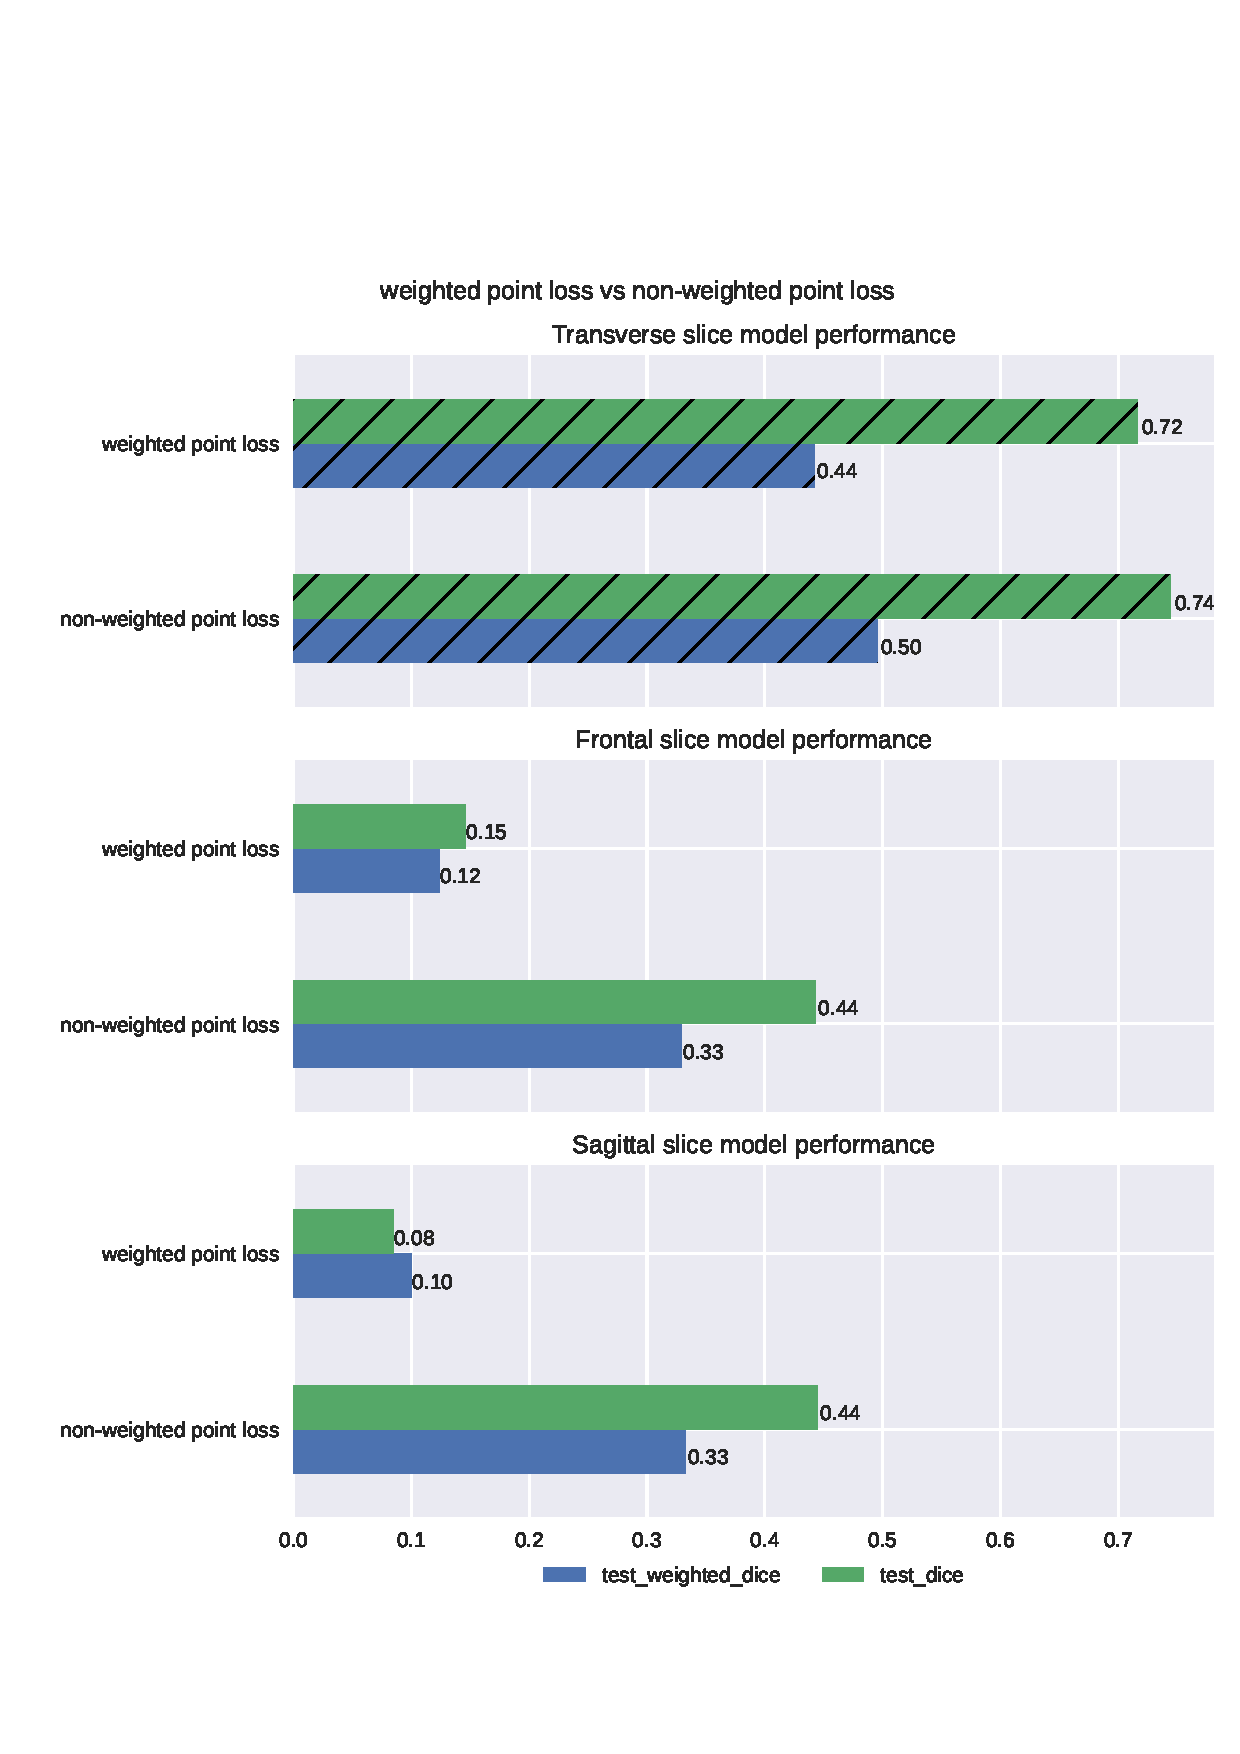
\includegraphics[width=.95\textwidth]{images/weightedvsnonweighted.png}
    \caption{Illustration of the difference in model performance between a weighted point loss function and the unweighted point loss function\label{fig:weighted_vs_unweighted}}
\end{SCfigure}

\subsubsection{Value of the added loss components}
\par{
    In this work, two loss components were added to the consistency loss published in \cite{Laradji}.
    The four loss components used in this work are described in more detail in \ref{sec:LossFunctions}.
    Where \cite{Laradji} is based only on the point loss $\mathcal{L}_P$ and the consistency loss $\mathcal{L}_C$, this work makes use of two extra loss components:
    the prior extend loss $\mathcal{L}_E$ and the separation loss $\mathcal{L}_S$.
    Figure \ref{fig:addedLossComponents} shows experimental results validating the positive influence these added loss terms have on the model performance.
}


\begin{SCfigure}[][htb]
    \centering
    \includegraphics[width=.95\textwidth]{images/TransverseModel_Losscomponents.png}
    \caption{Evaluation of the added value of loss components. \label{fig:addedLossComponents}}
\end{SCfigure}

\subsection{Evolution of the model performance with increased labelling effort}
\par{
    Probably the most basic modelling hyperparameter for a point annotation modelling campaign is the number of labelling points one asks the expert to provide.
    This section presents experimental results to estimate the influence of the number of annotation points on the resulting model performance.
    Intuitively, one would expect the model performance increases with the number of annotation points provided.
    This turns out to be false.
}


\chapter{Single dimension model combination\label{sec:combination}}
In chapter \ref{sec:singleDimension}, the construction of single dimension models is discussed.
These models extimate the segmentation masks of $352\times 352$ patches of scan volume slices along one of the three main axis.
In this chapter, the results of these single dimension models are combined to form a \textit{pseudo} mask that is subsequently used as labelling to train the final segmentation network.
Interesting to note in this procedure is that the evaluation metric of these obtained segmentation masks is improved in each of these steps.
The pseudo mask volume performs better than the single dimension model results and the final model trained on the pseudo masks performs better than the pseudo mask itself. 

\section{Volume combination procedure}
To construct one pseudo mask volume, first, three single dimension model are evaluated to form three stacks of two dimensional estimated segmentation masks, which are then combined to form three segmentation volumes. 
The resulting set of three segmentation volumes is then combined to form a new segmentation volume.
It is this last segmentation volume, made out of the combination, that is sliced again to obtain the pseudo masks for the final model.

\subsection{Recombination of the crops to slices}
All models are designed for $352 \times 352$ crops of the 2D slices\footnote{More information on the cropping of the slices can be found in chapter \ref{sec:cropping} on page \pageref{sec:cropping}.}.
To construct a segmentation volume from a single dimensional model, all relevant\footnote{Some slices have dimensions that do not allow to extract 5 different $352 \times 352$ crops. See for example figure \ref{fig:smallcrop} on page \pageref{fig:smallcrop}.} crops of each volume slice are evaluated.
First the segmentation results on these crops have to be combined again to obtain a segmentation mask of the whole slice.
Due to the cropping procedure, different crops of the same slice always partly overlap.
The crops are combined by averaging the logits $z_i$ for the overlapping positions.
The inferred class is then obtained from the resulting average $z_i$ values for that position. 

\subsection{Rule based result combination}
Once a stack of class segmentation masks for all slices of a volume are obtained, these can be combined to form a segmentation volumes.
Combining the results of three different single dimension models is performed in two steps:
\begin{enumerate}
    \item The resulting classification volumes are first combined with a rule-based method.
    \item After this rule-based combination, the resulting segmentation estimation is smoothened with a morphological filter.
\end{enumerate}

Three single dimension models are trained:
\begin{description}
    \item[Transverse slices] offer little context to indicate which of the lumbar vertebrae they contain. 
    It does not seem easy even for a human expert to indicate which vertebra is visible on the slice.
    The model trained on these slices is intended only for semantic segmentation.
    Each pixel is inferred only if it represents a vertebra, without distinction between the different lumbar vertebrae. 
    \item[Sagittal \& Coronal slices] do offer the necessary context to distinguish between $L_1$ to $L_5$. 
    The models trained on these slices do indicate the specific lumbar vertebra index. 
\end{description}

The volume combination rules are based on two observations:\footnote{
    The resulting estimations from a model for an input volume is again a three-dimensional volume ($\in \mathbb{N}^3$) with the same dimensions.
}.
\begin{enumerate}
    \item The precision (see equation \ref{eq:precision_i} on page \pageref{eq:precision_i}) with which the background class is predicted in all models is very high.
            This means $\mathcal{P} \left( label = background \mid prediction = background \right)$ is high for all models. 
            If there is one model that indicates a position is background, this position could be estimated to be background with high probability.
    \item The rule mentioned above can be nuanced\footnote{The opportunity to use the results of the other two single dimension models to correct a \textit{lapse} of one of the single dimension models can be recognized as one of the strengths of the combination procedure.}.
    It was observed that single dimension models can miss the mask\footnote{This is caused by the large differences between the different datasets used, see chapter \ref{sec:datasets} at page \pageref{sec:datasets}.}. 
    For some volumes, the recall of the vertebra class is extremely low. The single dimension model predicts the background class for allmost all positions.
    When this is observed, it does not make much sense to stick to the first rule.
\end{enumerate}
The observations mentioned above can be combined in algorithm \ref{alg:combination}.

\subsection{Morphological smoothing}
After the rule-based combination of estimations from different single dimension models, the result is smoothened with standard morphological filters.
These filters are combinations of the morphological \textit{erosion} and \textit{dilation} operators\footnote{
    This document is not intended to provide an elaborate explanation on morphological operations.
    For the readers conventience, the following symbolic notations are repeated:
    \begin{description}
        \item[Erosion] of set $\mathbf{A}$ by structural element $\mathbf{B}$ : $\mathbf{A} \ominus \mathbf{B}$ 
        \item[Dilation] of set $\mathbf{A}$ by structural element $\mathbf{B}$ : $\mathbf{A} \oplus \mathbf{B}$ 
        \item[Opening] of set $\mathbf{A}$ by structural element $\mathbf{B}$ : $\mathbf{A} \circ \mathbf{B} = (\mathbf{A} \ominus \mathbf{B}) \oplus \mathbf{B}$
        \item[Closing] of set $\mathbf{A}$ by structural element $\mathbf{B}$ : $\mathbf{A} \bullet \mathbf{B} = (\mathbf{A} \oplus \mathbf{B}) \ominus \mathbf{B}$
    \end{description}
}.

\begin{itemize}
    \item Noise in the single dimension segmentation masks is suppressed with an opening operation on the individual segmentation volumes of the single dimension models.
    \item Noise in the combined volumes is suppressed by first opening and then closing the volumes.
    \item The estimated volumes are observed to overestimate the extent of the vertebrae. For this reason, an erosion step is performed to decrease the overall extent of the class masks.
\end{itemize}

The procedure mentioned above has two hyperparameters: the number of iterations for the denoising filters and the number of iterations for the erosion filter.
Both hyperparameters are estimated by calculating the same evaluation metric, the weighted dice score on the validation set, as for the single-dimensional model evaluation. 

\subsection{Volume combination algorithm}
The combination of the rules and morphological smoothing operations discussed above result in the following algorithm to combine the segmentation volumes from the single dimension models\footnote{
    The cardinality of a set $\mathbf{A}$, written as $|\mathbf{A}|$, is the number of elements in a set.
    The cardinality of the class label sets $c_.$ thus represents the voxel count in each segmentation volumes that is estimated to be \textit{not background}.
    Suspiciously low voxel counts classified other than background are defined as lower than 35\% of the highest class label cardinality.
    This last factor has not been optimised. It is an engineering estimate.
    If a volume is found to be have such a low class label cardinality, this volume reference is stored as $d_{ignore}$ and the volume is ignore in the combination protocol.
    In practice, the low cardinality volumes are all the segmentation volumes obtained from the model trained on point annotated tranverse slices.
}:

\begin{algorithm}[H]
    \SetAlgoLined
    \KwData{
        Results $y_.$ of three models indicating an estimated class for all positions $\vec{p}$ in the volume. \;
        Transverse model $y_t \in \mathbb{N}^3: \forall y_t(\vec{p}) \in \{ 0, 1 \}$ \;
        Sagittal model $y_s \in \mathbb{N}^3: \forall y_t(\vec{p}) \in \{ 0, 1, 2, 3, 4, 5 \}$ \;
        Coronal model $y_c \in \mathbb{N}^3: \forall y_t(\vec{p}) \in \{ 0, 1, 2, 3, 4, 5 \}$  \;
        Binary $\mathbf{B}$ structure with rank 3 and connectivity 3 \;
    }
    \KwResult{Combination of the three model results $y_f$.}
    \tcp{Closing operation on all $y_.$}
    $y_t \leftarrow y_t \bullet \mathbf{B}$ \;
    $y_s \leftarrow y_s \bullet \mathbf{B}$ \;
    $y_c \leftarrow y_c \bullet \mathbf{B}$ \;
    \tcp{(relative) cardinality of the class label sets}
    $c_t \leftarrow |\{ y_t \neq 0 \}|$ \;
    $c_s \leftarrow |\{ y_s \neq 0 \}|$ \;
    $c_c \leftarrow |\{ y_c \neq 0 \}|$ \;
    $r_t \leftarrow \frac{c_t}{max(c_t, c_s, c_c)}$ \;
    $r_s \leftarrow \frac{c_s}{max(c_t, c_s, c_c)}$ \;
    $r_c \leftarrow \frac{c_c}{max(c_t, c_s, c_c)}$ \;
    \lIf{$\exists d \in [ t,s,c ] : r_d < 0.35$}{$d_{ignore} \leftarrow d$}\lElse{$d_{ignore} \leftarrow \emptyset$}
    \For{all $\vec{p}$}{
        $i \in [ 1, 2, 3, 4, 5]$ \;
        \Switch{$d_{ignore}$}{
            \Case{$\emptyset$}{
                \lIf{$y_t[\vec{p}] = 1 \wedge y_s[\vec{p}] = i \wedge y_c[\vec{p}] = i$}{
                    $y_f[\vec{p}] \leftarrow i$ 
                }
                \lElse{
                    $y_f[\vec{p}] \leftarrow 0$ 
                }
            }
            \Case{$t$}{
                \lIf{$y_s[\vec{p}] = i \wedge y_c[\vec{p}] = i$}{
                    $y_f[\vec{p}] \leftarrow i$ 
                }
                \lElse{
                    $y_f[\vec{p}] \leftarrow 0$
                }
            }
            \Case{$s$}{
                \lIf{$y_t[\vec{p}] = 1 \wedge y_c[\vec{p}] = i$}{
                    $y_f[\vec{p}] \leftarrow i$ 
                }
                \lElse{
                    $y_f[\vec{p}] \leftarrow 0$ 
                }
            }
            \Case{$c$}{
                \lIf{$y_t[\vec{p}] = 1 \wedge y_s[\vec{p}] = i$}{
                    $y_f[\vec{p}] \leftarrow i$ 
                }
                \lElse{
                    $y_f[\vec{p}] \leftarrow 0$ 
                }
            }
        }
    }
    $y_f \leftarrow ((y_f \circ \mathbf{B}) \bullet \mathbf{B}) \ominus \mathbf{B}$
   \caption{Rule based combination of model results from three single dimension models\label{alg:combination}}
\end{algorithm}

\section{Pseudo mask performance}
Using algorithm \ref{alg:combination}, a segmentation volume can be obtained with a higher weighted dice metric than the each of the individual segmentation volumes obtained from the single dimension models.
This is tested by combining three models.
Table \ref{tab:combination_1} illustrates this concept.

\begin{SCtable}[\sidecaptionrelwidth][h]

    \begin{tabular}{l|lll}
        \hline
        \textbf{\begin{tabular}[c]{@{}l@{}}Slice \\ direction\end{tabular}} &
          \textbf{Transverse} &
          \textbf{Coronal} &
          \textbf{Sagittal} \\ \hline
        \begin{tabular}[c]{@{}l@{}}Context\\ Slices {[}mm{]}\end{tabular}   & 1     & 1     & 1     \\ \cline{1-1}
        \begin{tabular}[c]{@{}l@{}}Points per\\ class instance\end{tabular} & 1     & 1     & 1     \\ \cline{1-1}
        \begin{tabular}[c]{@{}l@{}}Background \\ points\end{tabular}        & 5     & 3     & 3     \\ \cline{1-1}
        Dataset &
          \begin{tabular}[c]{@{}l@{}}PLoS\\ xVertSeg\\ USiegen\\ MyoSegmenTUM\end{tabular} &
          \multicolumn{2}{l}{\begin{tabular}[c]{@{}l@{}}xVertSeg\\ USiegen\\ MyoSegmenTUM\end{tabular}} \\ \cline{1-1}
        \begin{tabular}[c]{@{}l@{}}Segmentation\\ classes\end{tabular}      & 2     & 6     & 6     \\ \cline{1-1}
        \begin{tabular}[c]{@{}l@{}}Weighted \\ dice score\end{tabular}      & 0.476 & 0.339 & 0.350 \\ \hline
        \begin{tabular}[c]{@{}l@{}}Weighted\\ dice score\\ combination\end{tabular} &
          \multicolumn{3}{c}{\textit{0.51}} \\ \hline
        \end{tabular}
    \caption{Combination of three point supervised models with algorithm \ref{alg:combination}. 
    These models were constructed with a fixed number of background points and a fixed number of class labels per class instance.
    This test indicates that the segmentation mask obtained from the result of single dimension models with algorithm \ref{alg:combination} allows to obtain a new segmentation mask with a higher metric score, the pseudo masks.
    Pay attention, the weighted dice scores for the individual models are evaluated on the test set, while the weighted dice score for the combination is evaluated on the cross validation set. \label{tab:combination_1}
    }

\end{SCtable}

In table \ref{combination_1}, the segmentation quality is calculated on the validation set.
Since there are two hyperparameters (the number of denoise iterations and the number of erosion iterations) to optimise in the combination algorithm \ref{alg:combination}, 
the algorithm is evaluated with a matrix of these hyperparameters and 

\marginpar{
        \includegraphics{images/combination_optimization_1.png}
        \captionof{figure}{Illustration of the hyperparameter optimization procedure for the combination detailed in \ref{combination_1}}
        \label{fig:hyperparameter_combination_1}
    }

\begin{SCfigure}[][htb]
    \centering
    \includegraphics[width=.95\textwidth]{images/morphmask_denoise1_erode1_MyoSegmenTUM_036.png}
    \caption{
        Result of the combination of the three single dimension model results for volume MyoSegmenTUM nr 43.
        The colours indicate the vertebra classes. Only one semantic class is estimated in the first row, illustrating the model trained on transversal slices.
        On the first three rows, slices of the resulting segmentations from the single dimension models are shown. 
        It is clear these masks contain some artefacts and are not always in agreement with each other.
        On the fourth row, the result after mask combination and morphological smoothing is shown. 
        This corresponds more closely to the ground truth mask, shown on the fifth row.
        This final mask, shown on the fourth row, will be used as a pseudo mask to approximate the unknown ground truth mask.
        In the last row, the corresponding images are shown.
    }
\end{SCfigure}

\chapter{Pseudo mask training}

Time to evaluate
performance

\newgeometry{total={210mm,297mm},left=20mm,right=20mm,bindingoffset=5mm, top=25mm,bottom=25mm} 
\begin{partwithabstract}{Conclusions}
    This part of the document summarizes the most important conclusions from this work and possible ideas as a way forward after this work.
    The part starts with an evaluation and discussion of the labelling cost necessary to make the final model. 
    Finally, the lessons learned from this project are laid out and some ideas for further development of weakly supervised models for medical applications are presented. 
\end{partwithabstract}
\restoregeometry



\appendix

\newgeometry{total={210mm,297mm},left=30mm,right=30mm,bindingoffset=5mm, top=25mm,bottom=25mm}
\begin{partwithabstract}{Appendix}
  Apendices to the document:
  \begin{enumerate}
    \item Software environment used
    \item Agreement documents for use of two datasets.
  \end{enumerate}
\end{partwithabstract}
\restoregeometry
\chapter{Medical terms}

Clarification of the medical lingo used.

\begin{SCfigure}[][htb]
  \centering
  \includegraphics[width=10cm]{/home/thesis/images/Anatomical_Planes.png}
  \caption{Clarification of the terms regarding the anatomical planes
  }
\end{SCfigure}

\begin{SCfigure}[][htb]
  \centering
  \includegraphics[width=10cm]{/home/thesis/images/prone_supine.png}
  \caption{Supine (face-up) and Prone (face-down) position of a patient.}
\end{SCfigure}

\chapter{Used software}

\todo[inline]{Software environments can be build with dockerfiles available in folder \textit{/dockerfiles/code/} of the git.}

\todo[inline]{Assure proper referencing of all libraries used}

\begin{SCtable}[\sidecaptionrelwidth][h]
 
  \begin{tabular}{ p{6cm} l l } 
   \hline
   \hline
   Library & version & reference  \\
   \hline 
   PyTorch & 1.7.1 &  \\ 
   SimpleITK &  &  \\ 
   \hline
   \hline
  \end{tabular}
  \caption{Python libraries used}

\end{SCtable}
\newgeometry{total={210mm,297mm},left=30mm,right=30mm,bindingoffset=5mm, top=25mm,bottom=25mm}
\chapter{Dataset agreements\label{seg:datasetagreement}}

\includegraphics[width=17cm]{/home/thesis/images/AgreementxVertSeg.png}

%\nocite{*} 
\printbibliography

\clearpage\null\newpage


\end{document}

